%%%%%%%%%%%%%%%%%%%%%%%%%%%%%%%%%%%%%%%%%%%%%%%%%%%%%%%%%%%%%%%%%%%%%%%%%%%%%%%%%%
\begin{frame}[fragile]\frametitle{}
\begin{center}
{\Large Retrieval Augmented Generation (RAG)}
\end{center}
\end{frame}

%%%%%%%%%%%%%%%%%%%%%%%%%%%%%%%%%%%%%%%%%%%%%%%%%%%%%%%%%%%
\begin{frame}[fragile]\frametitle{Quiz}
  \begin{itemize}
    \item How to do domain adaptation? ie
	\item How to build custom LLM solution? meaning
	\item How can LLM based chatbot answer from my data?
  \end{itemize}
  
  Answers??
  
\end{frame}

%%%%%%%%%%%%%%%%%%%%%%%%%%%%%%%%%%%%%%%%%%%%%%%%%%%%%%%%%%%
\begin{frame}[fragile]\frametitle{Need for Domain Adaptation}

\begin{itemize}
\item Industrial settings prioritize cost, privacy, and reliability of solutions.
\item LLMs are prone to hallucinations, factual errors, and looping.
\item LLMs need to work on own/private/streaming/latest data
\item Speed/latency/efficiency Concerns
\item Solution: To build LLM from scratch?? needs?? 
\item Extensive training data, high computational resources and \$\$\$\$
% \item RAG vs Fine-tuning
% \item Companies, including startups, seek solutions with a return on investment rather than investing in talent or training models from scratch.
% \item Recent research and chatbot releases demonstrate the capability to leverage knowledge beyond model weights.
% \item One approach is to iteratively call another neural network or language model (LM) to extract required information.
% \item Iteratively calling LM involves multiple interactions to extract information as shown in the provided image.g, as separating reasoning from factual information is not straightforward.
\end{itemize}	

So, what to do?

\end{frame}

%%%%%%%%%%%%%%%%%%%%%%%%%%%%%%%%%%%%%%%%%%%%%%%%%%%%%%%%%%%
\begin{frame}[fragile]\frametitle{Training and Query Mismatch}


		\begin{center}
		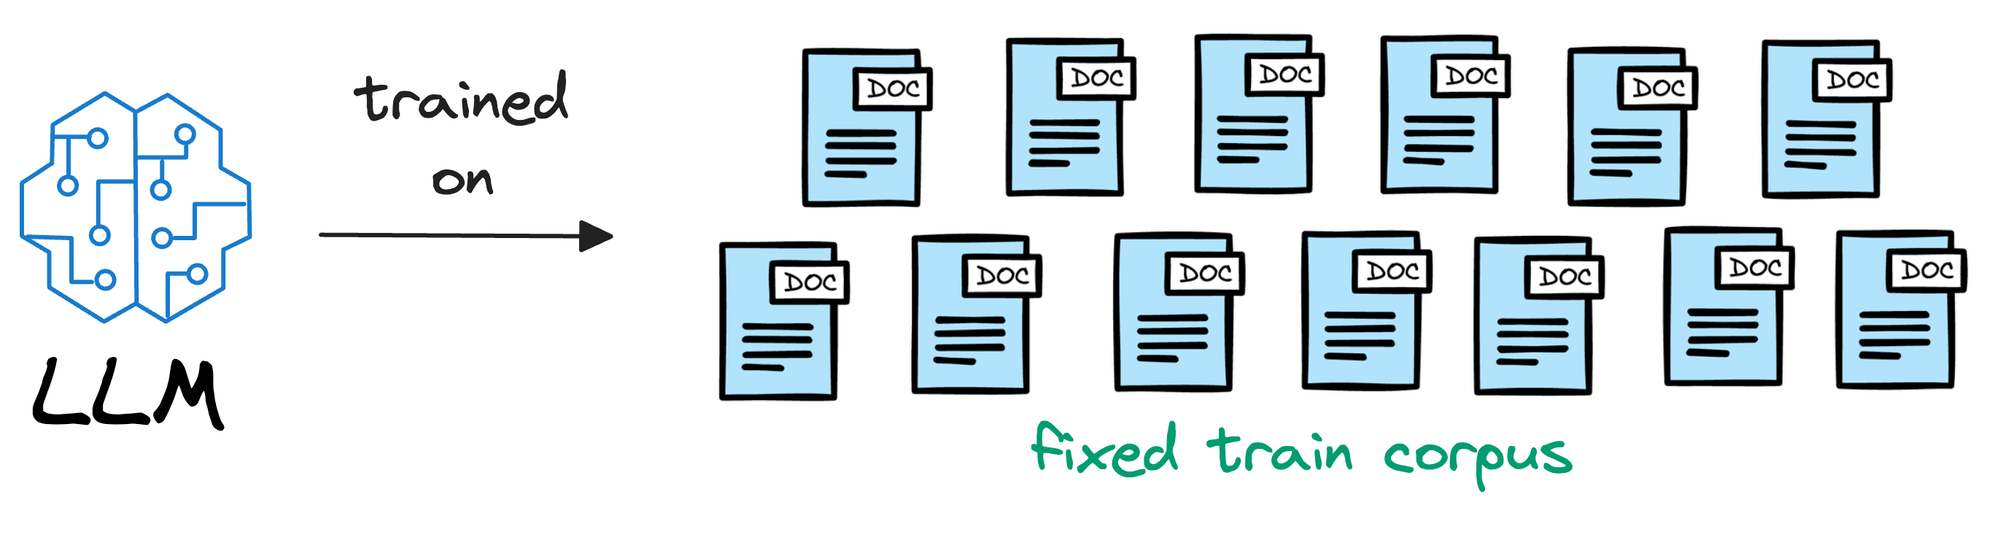
\includegraphics[width=\linewidth,keepaspectratio]{rag44}
		
		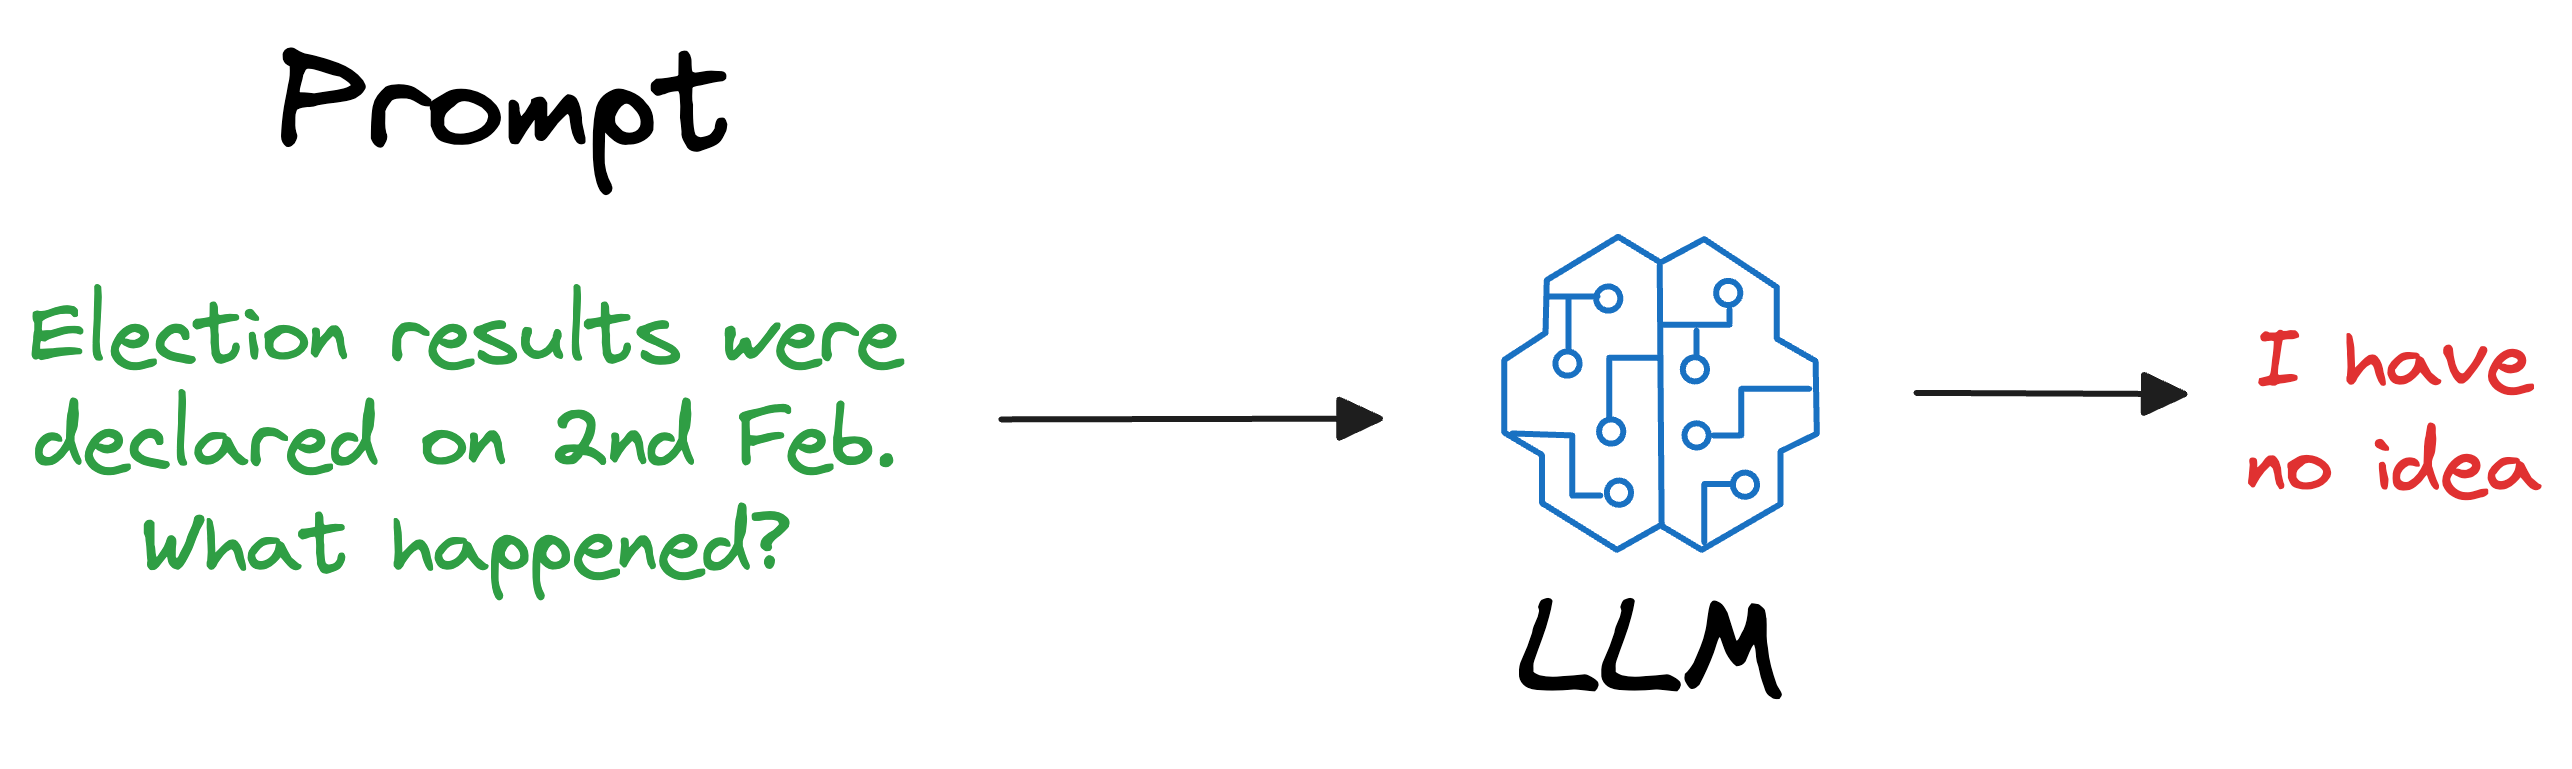
\includegraphics[width=\linewidth,keepaspectratio]{rag45}
		
		\end{center}

{\tiny (Ref: A Crash Course on Building RAG Systems -Daily Dose)}

\end{frame}


%%%%%%%%%%%%%%%%%%%%%%%%%%%%%%%%%%%%%%%%%%%%%%%%%%%%%%%%%%%
\begin{frame}[fragile]\frametitle{Solutions}
  \begin{itemize}
    \item Few Shots
	\item RAG
	\item Fine-tuning
  \end{itemize}
\end{frame}


% %%%%%%%%%%%%%%%%%%%%%%%%%%%%%%%%%%%%%%%%%%%%%%%%%%%%%%%%%%%
% \begin{frame}[fragile]\frametitle{Introduction}

% \begin{itemize}
% \item What is RAG? A new paradigm for generation tasks, combining retrieval and generation models.
% \item Motivation: Overcoming limitations of pure generative models in factual consistency, efficiency, and diversity.
% \item Impact: Improved performance in text summarization, question answering, and other NLP tasks.
% \end{itemize}	

% \end{frame}


% %%%%%%%%%%%%%%%%%%%%%%%%%%%%%%%%%%%%%%%%%%%%%%%%%%%%%%%%%%%
% \begin{frame}[fragile]\frametitle{RAG in Iterations}


% \begin{center}
% \includegraphics[width=0.8\linewidth,keepaspectratio]{chatgpt46}
% \end{center}

% {\tiny (Ref: Overview of Large Language Models - Aman AI)}

% \end{frame}

%%%%%%%%%%%%%%%%%%%%%%%%%%%%%%%%%%%%%%%%%%%%%%%%%%%%%%%%%%%
\begin{frame}[fragile]\frametitle{Why RAG?}
\begin{itemize}
  \item \textbf{Unlimited Knowledge:}
    \begin{itemize}
      \item RAG enables access external sources, surpassing limitations of its data.
      \item Allows exploration of proprietary documents and internet searches%, broadening understanding.
      % \item Introduces both Parametric and Non-Parametric Memory, enhancing models' knowledge.
      % \item Read the seminal paper on RAG - https://lnkd.in/gN2cAcXx.
    \end{itemize}
  
  \item \textbf{Easier to Update/Maintain:}
    \begin{itemize}
      \item Offers a cost-effective way to update and maintain %non-parametric memory in LLMs.
      \item Building a knowledge base minimizes ongoing maintenance financial burden.
      % \item Pre-training expenses are mitigated, and fine-tuning is tailored to specific use cases.
      % \item Read Gopi's blog on cost implications of LLMs - https://lnkd.in/gJ-bT4RH.
    \end{itemize}
	
  \item \textbf{Confidence in Responses:}
    \begin{itemize}
      \item Enhances confidence by providing extra context for more accurate responses.
      \item Practical boost to overall intelligence in generating responses.
    \end{itemize}	
% \end{itemize}

% \end{frame}

% %%%%%%%%%%%%%%%%%%%%%%%%%%%%%%%%%%%%%%%%%%%%%%%%%%%%%%%%%%%
% \begin{frame}[fragile]\frametitle{Why RAG? contd.}

% \begin{itemize}
  % \item \textbf{Context Awareness:}
    % \begin{itemize}
      % \item RAG makes LLMs adept at understanding context through added information.
      % \item Results in responses that are not only accurate but also contextually fitting.
    % \end{itemize}

  \item \textbf{Source Citation:}
    \begin{itemize}
      \item RAG provides access to sources, improving transparency in LLM responses.
      \item A step towards building trust in LLM systems.
      % \item Explore text generation with citations in LLMs - Perplexity, Microsoft Co Pilot % https://lnkd.in/g2VEwRBK.
    \end{itemize}

  \item \textbf{Reduced Hallucinations:}
    \begin{itemize}
      \item RAG-enabled LLMs exhibit reduced creative misfires.
      \item Solid foundation of information keeps models focused and grounded.
      % \item Pinecone explains more in this post - https://lnkd.in/gCfkDZYp.
    \end{itemize}

  % \item \textbf{Practical Empowerment:}
    % \begin{itemize}
      % \item RAG shifts how we empower LLM systems practically.
      % \item Focuses on expanding knowledge, building confidence, and maintaining grounded responses.
    % \end{itemize}
\end{itemize}

\end{frame}

% %%%%%%%%%%%%%%%%%%%%%%%%%%%%%%%%%%%%%%%%%%%%%%%%%%%%%%%%%%%
% \begin{frame}[fragile]\frametitle{History of RAG (Retrieval-Augmented Generation)}
  % \begin{itemize}
    % \item RAG, or Retrieval-Augmented Generation, was introduced by Meta in a paper addressing limitations of large pre-trained language models.
    % \item Big language models struggled with effectively accessing and manipulating knowledge, especially in tasks heavy on knowledge.
    % \item Challenges included difficulty explaining decisions and keeping up with real-world changes.
  % \end{itemize}
% \end{frame}

% %%%%%%%%%%%%%%%%%%%%%%%%%%%%%%%%%%%%%%%%%%%%%%%%%%%%%%%%%%%
% \begin{frame}[fragile]\frametitle{History of RAG (Retrieval-Augmented Generation)}

% \begin{center}
% \includegraphics[width=\linewidth,keepaspectratio]{llm132}
% \end{center}				


% https://arxiv.org/pdf/2005.11401.pdf

% {\tiny (Ref: Applied LLMs Mastery 2024 - Aishwarya Reganti)}

% \end{frame}

% %%%%%%%%%%%%%%%%%%%%%%%%%%%%%%%%%%%%%%%%%%%%%%%%%%%%%%%%%%%
% \begin{frame}[fragile]\frametitle{Challenges in Existing Models}
  % \begin{itemize}
    % \item Before RAG, hybrid models like REALM and ORQA showed promise by combining parametric and non-parametric memories.
    % \item These models integrated masked language models with a retriever, demonstrating positive outcomes in handling knowledge-intensive tasks.
  % \end{itemize}
% \end{frame}

% %%%%%%%%%%%%%%%%%%%%%%%%%%%%%%%%%%%%%%%%%%%%%%%%%%%%%%%%%%%
% \begin{frame}[fragile]\frametitle{Introduction of RAG}
  % \begin{itemize}
    % \item RAG emerged as a flexible fine-tuning method for retrieval-augmented generation.
    % \item It combined pre-trained parametric memory (seq2seq model) with non-parametric memory from a dense vector index of Wikipedia.
    % \item Access to non-parametric memory was facilitated through a pre-trained neural retriever like Dense Passage Retriever (DPR).
    % \item RAG aimed to enhance pre-trained, parametric-memory generation models by incorporating non-parametric memory through fine-tuning.
  % \end{itemize}
% \end{frame}


% %%%%%%%%%%%%%%%%%%%%%%%%%%%%%%%%%%%%%%%%%%%%%%%%%%%%%%%%%%%
% \begin{frame}[fragile]\frametitle{Introduction of RAG}
  % \begin{itemize}
    % \item RAG emerged as a flexible fine-tuning method for retrieval-augmented generation.
    % \item It combined pre-trained parametric memory (seq2seq model) with non-parametric memory from a dense vector index of Wikipedia.
    % \item Access to non-parametric memory was facilitated through a pre-trained neural retriever like Dense Passage Retriever (DPR).
    % \item RAG aimed to enhance pre-trained, parametric-memory generation models by incorporating non-parametric memory through fine-tuning.
  % \end{itemize}
% \end{frame}

% %%%%%%%%%%%%%%%%%%%%%%%%%%%%%%%%%%%%%%%%%%%%%%%%%%%%%%%%%%%
% \begin{frame}[fragile]\frametitle{Significance of RAG}
  % \begin{itemize}
    % \item RAG departed from past approaches by pre-training both parametric and non-parametric memory components with abundant knowledge.
    % \item It achieved top-notch results in open-domain question answering and surpassed previous models in fact verification and knowledge-intensive generation.
  % \end{itemize}
% \end{frame}

% %%%%%%%%%%%%%%%%%%%%%%%%%%%%%%%%%%%%%%%%%%%%%%%%%%%%%%%%%%%
% \begin{frame}[fragile]\frametitle{Adaptability and Achievements of RAG}
  % \begin{itemize}
    % \item RAG demonstrated adaptability by allowing the non-parametric memory to be swapped out and updated, keeping the model's knowledge fresh.
    % \item Notable achievements include excelling in open-domain question answering and outperforming in fact verification and knowledge-intensive generation.
  % \end{itemize}
% \end{frame}


%%%%%%%%%%%%%%%%%%%%%%%%%%%%%%%%%%%%%%%%%%%%%%%%%%%%%%%%%%%
\begin{frame}[fragile]\frametitle{Important Questions}
\begin{itemize}
  \item Does the use case require external data access?
  \item Does the use case require changing foundation model style?
  \item Does the use case require addressing hallucinations?
  \item Is labeled training data available?
  \item Is citing the source of information important?
  \item How critical is system latency?
  \item What are the cost implications?
  \item What are the scalability requirements?
  \item Do we have the necessary expertise?
\end{itemize}
\end{frame}



%%%%%%%%%%%%%%%%%%%%%%%%%%%%%%%%%%%%%%%%%%%%%%%%%%%%%%%%%%%%%%%%%%%%%%%%%%%%%%%%%%
\begin{frame}[fragile]\frametitle{}
\begin{center}
{\Large Retrieval Augmented Generation (RAG) Workflow}
\end{center}
\end{frame}

%%%%%%%%%%%%%%%%%%%%%%%%%%%%%%%%%%%%%%%%%%%%%%%%%%%%%%%%%%%
\begin{frame}[fragile]\frametitle{RAG Workflow}


		\begin{center}
		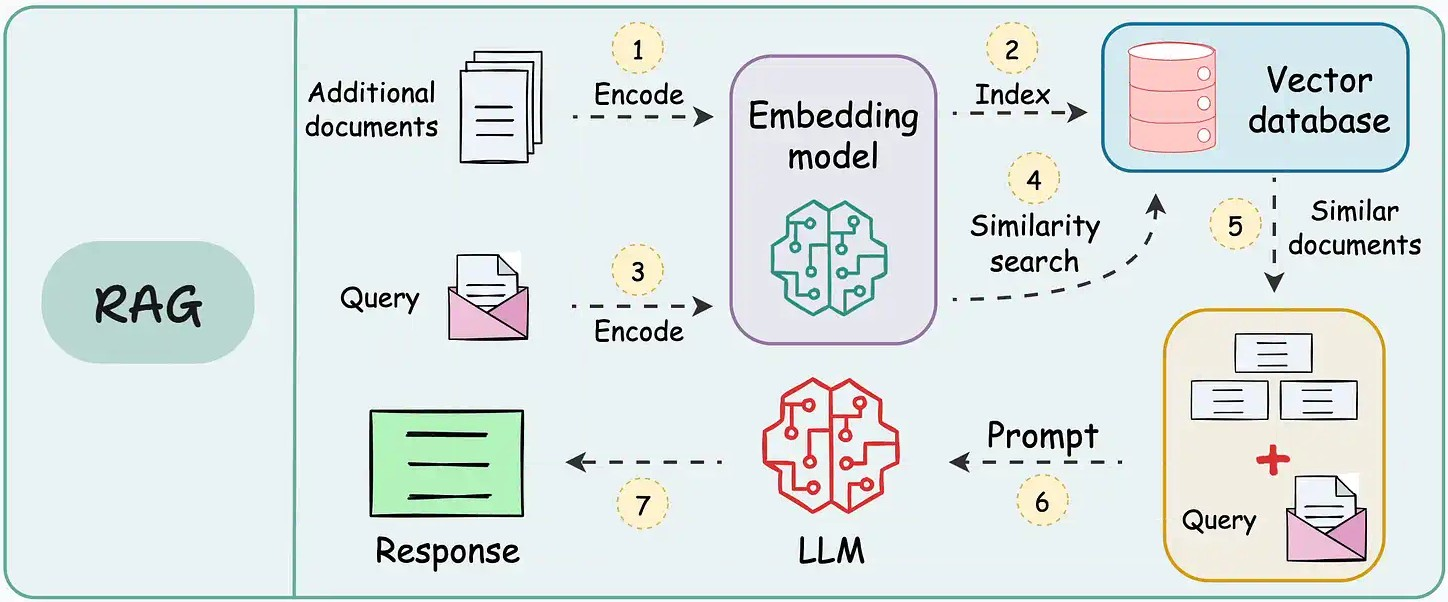
\includegraphics[width=\linewidth,keepaspectratio]{rag41}
		\end{center}

{\tiny (Ref: A Crash Course on Building RAG Systems -Daily Dose)}

\end{frame}


%%%%%%%%%%%%%%%%%%%%%%%%%%%%%%%%%%%%%%%%%%%%%%%%%%%%%%%%%%%
\begin{frame}[fragile]\frametitle{RAG Components}


		\begin{center}
		\includegraphics[width=0.8\linewidth,keepaspectratio]{rag36}
		\end{center}

{\tiny (Ref: [Week 4] Retrieval Augmented Generation -Aishwarya Naresh Reganti)}

\end{frame}

%%%%%%%%%%%%%%%%%%%%%%%%%%%%%%%%%%%%%%%%%%%%%%%%%%%%%%%%%%%
\begin{frame}[fragile]\frametitle{RAG Components}


\begin{itemize}
  \item Ingestion:
	\begin{itemize}
	  \item Documents undergo segmentation into chunks, and embeddings are generated from these chunks, subsequently stored in an index.
	  \item Chunks are essential for pinpointing the relevant information in response to a given query, resembling a standard retrieval approach.
	  \end{itemize}

  \item Retrieval:
	\begin{itemize}
	  \item Leveraging the index of embeddings, the system retrieves the top-k documents when a query is received, based on the similarity of embeddings.
	\end{itemize}
	  
  \item Synthesis:
	\begin{itemize}
	  \item Examining the chunks as contextual information, the LLM utilizes this knowledge to formulate accurate responses.
	\end{itemize}

\end{itemize}

\end{frame}

%%%%%%%%%%%%%%%%%%%%%%%%%%%%%%%%%%%%%%%%%%%%%%%%%%%%%%%%%%%
\begin{frame}[fragile]\frametitle{Create chunks}



		\begin{center}
		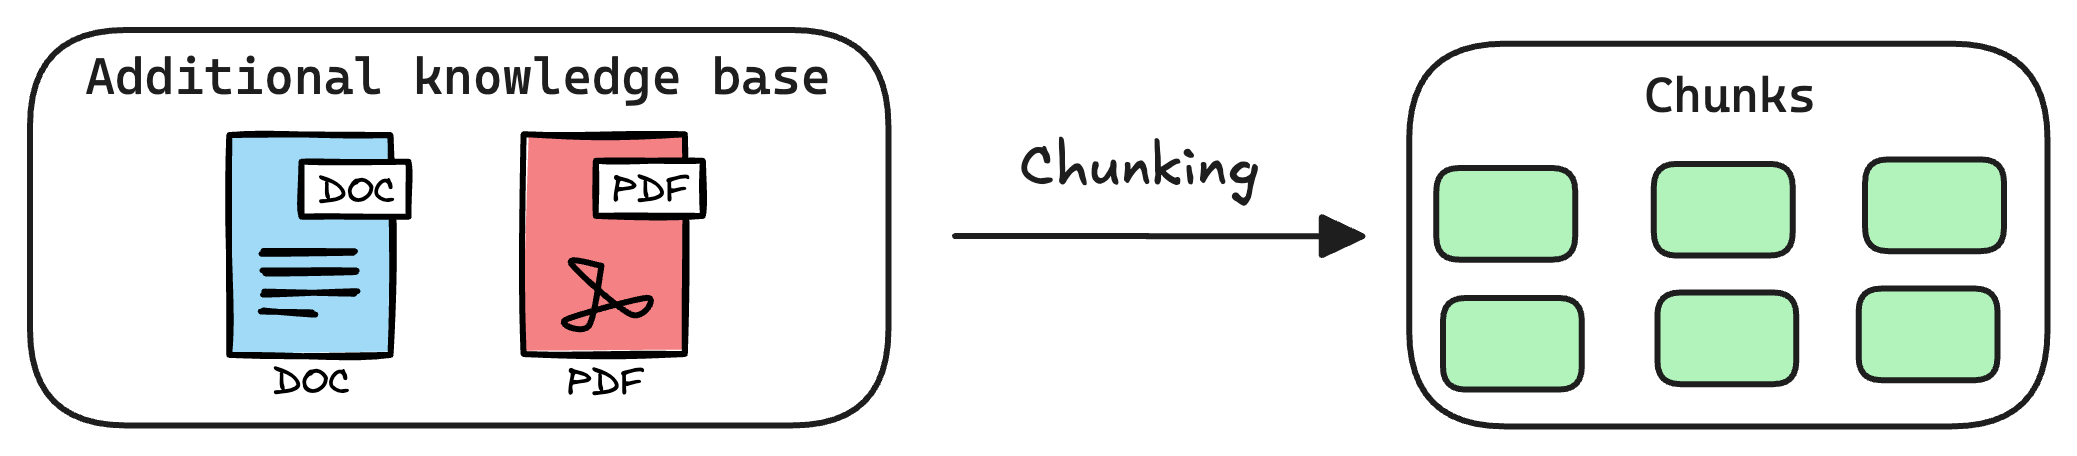
\includegraphics[width=\linewidth,keepaspectratio]{rag50}
		
		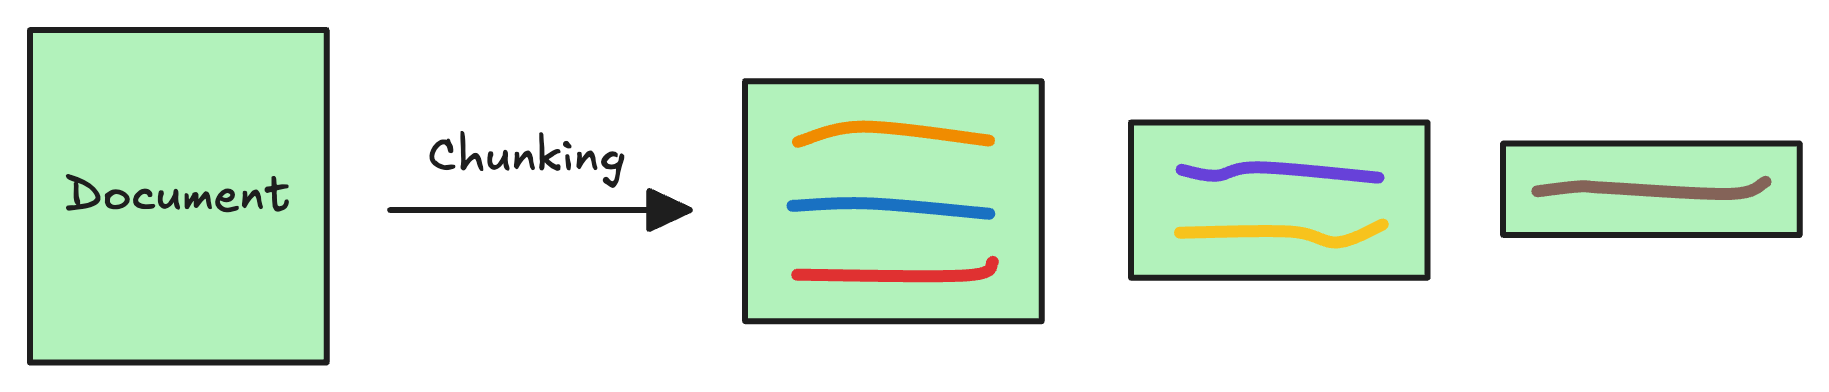
\includegraphics[width=\linewidth,keepaspectratio]{rag51}
		
		\end{center}

{\tiny (Ref: A Crash Course on Building RAG Systems -Daily Dose)}


\end{frame}


%%%%%%%%%%%%%%%%%%%%%%%%%%%%%%%%%%%%%%%%%%%%%%%%%%%%%%%%%%%
\begin{frame}[fragile]\frametitle{5 Chunking Strategies For RAG}



		\begin{center}
		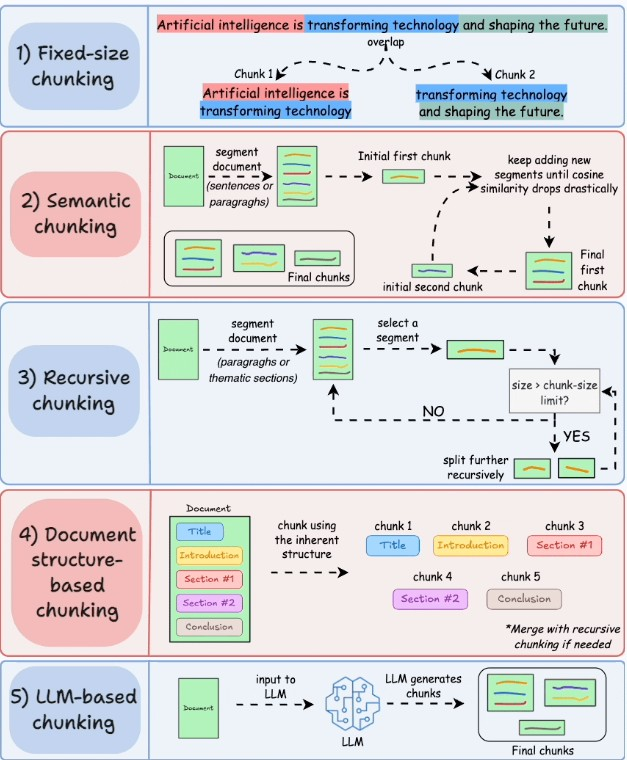
\includegraphics[width=0.5\linewidth,keepaspectratio]{rag52}
		
{\tiny (Ref: A Crash Course on Building RAG Systems -Daily Dose)}
		
	
		\end{center}



\end{frame}


%%%%%%%%%%%%%%%%%%%%%%%%%%%%%%%%%%%%%%%%%%%%%%%%%%%%%%%%%%%
\begin{frame}[fragile]\frametitle{Generate embeddings}



		\begin{center}
		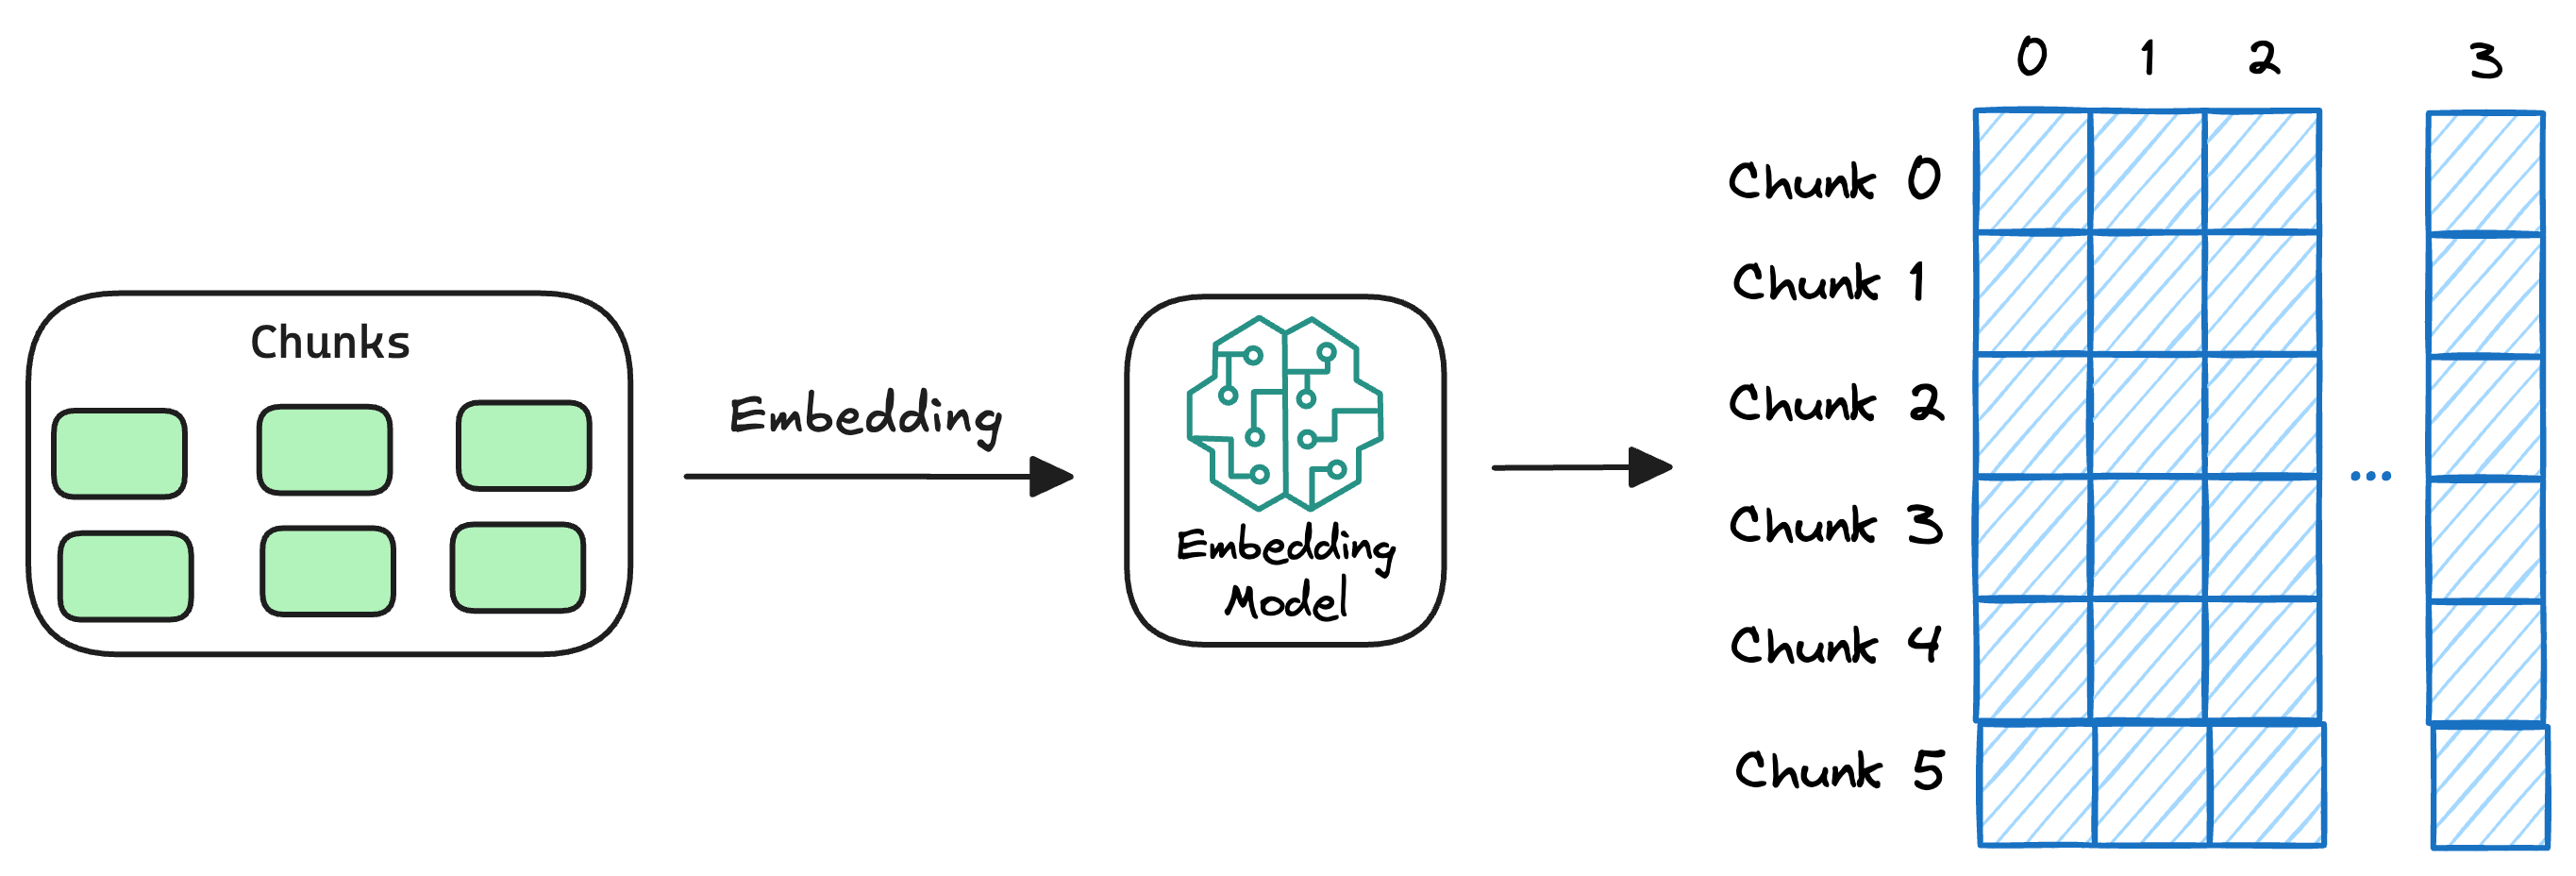
\includegraphics[width=0.8\linewidth,keepaspectratio]{rag53}
		
		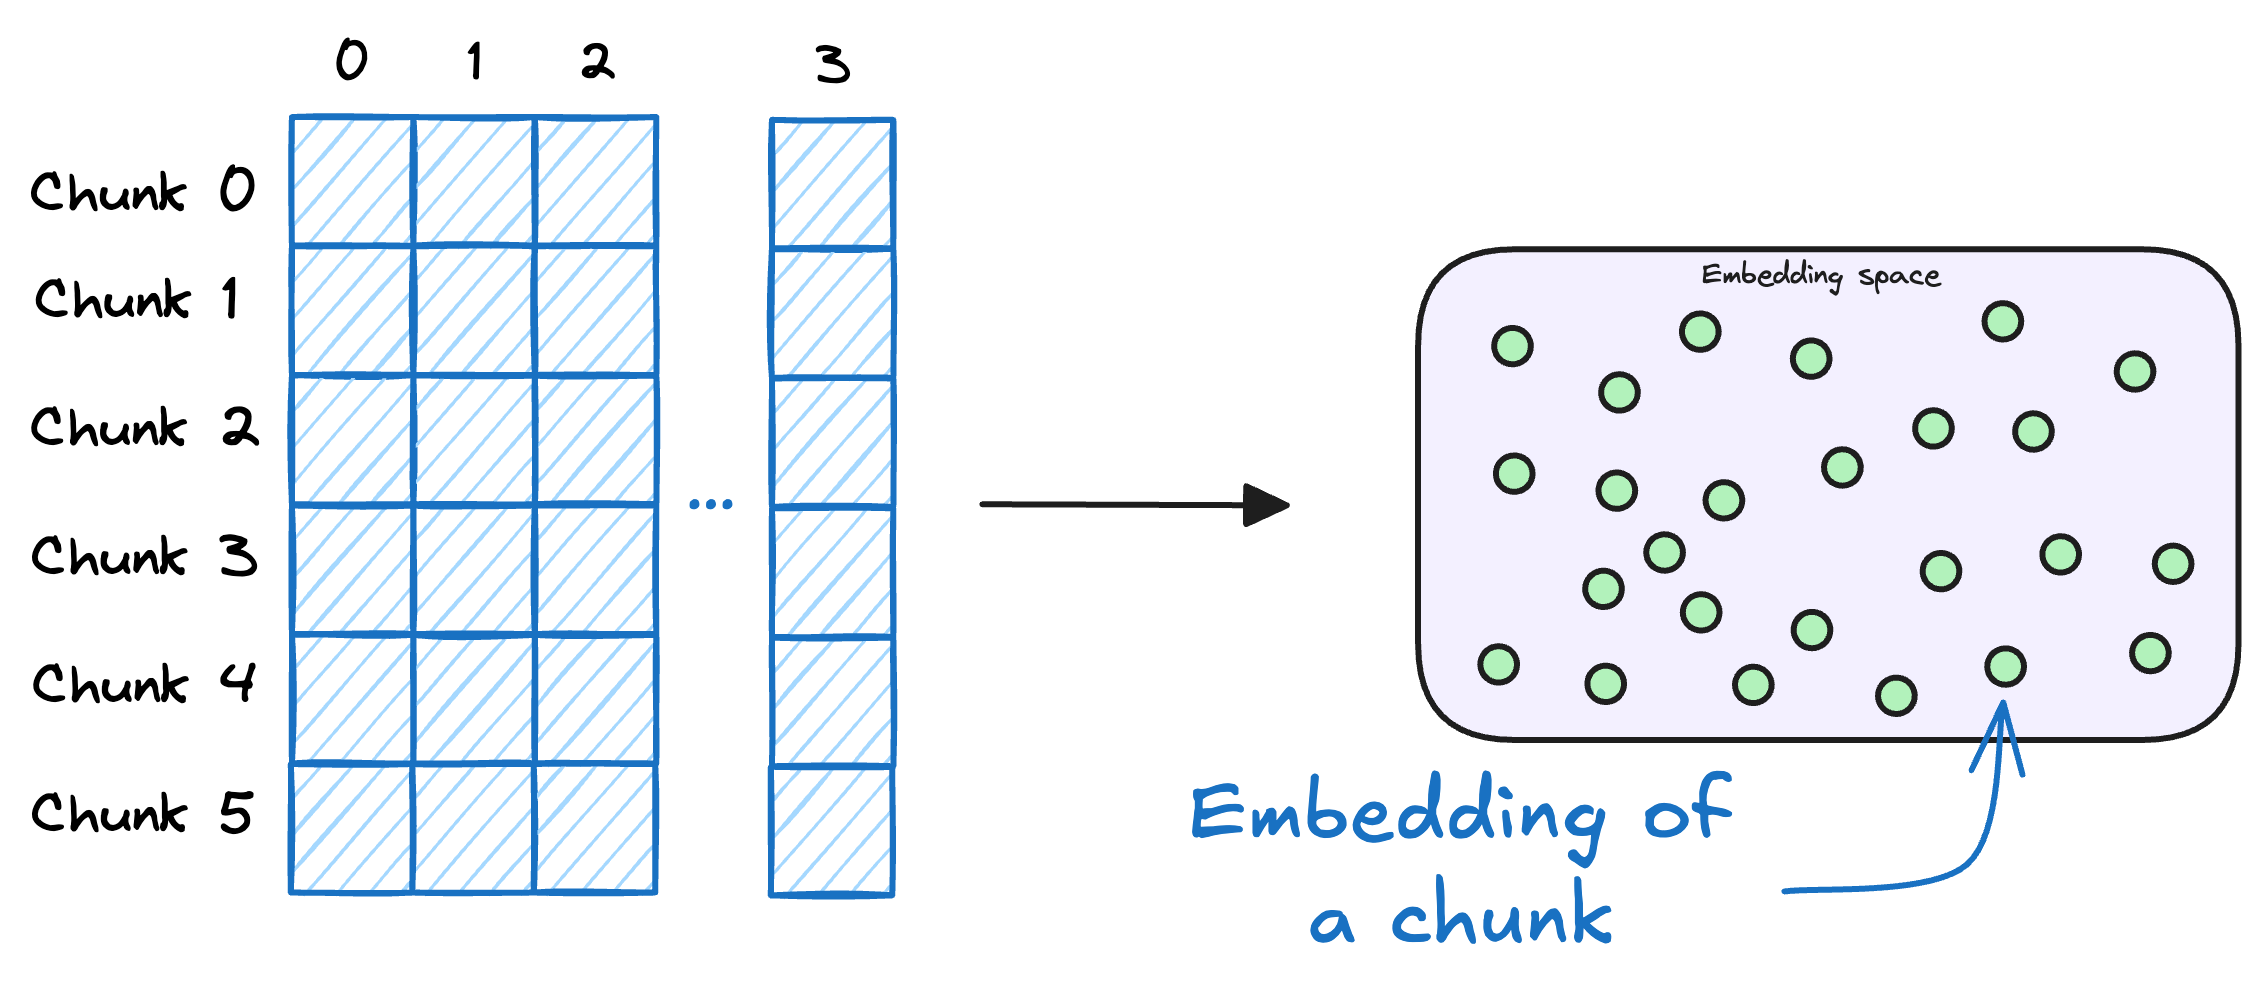
\includegraphics[width=0.8\linewidth,keepaspectratio]{rag54}
		
		\end{center}

{\tiny (Ref: A Crash Course on Building RAG Systems -Daily Dose)}


\end{frame}

%%%%%%%%%%%%%%%%%%%%%%%%%%%%%%%%%%%%%%%%%%%%%%%%%%%%%%%%%%%
\begin{frame}[fragile]\frametitle{Vector Databases}


		\begin{center}
		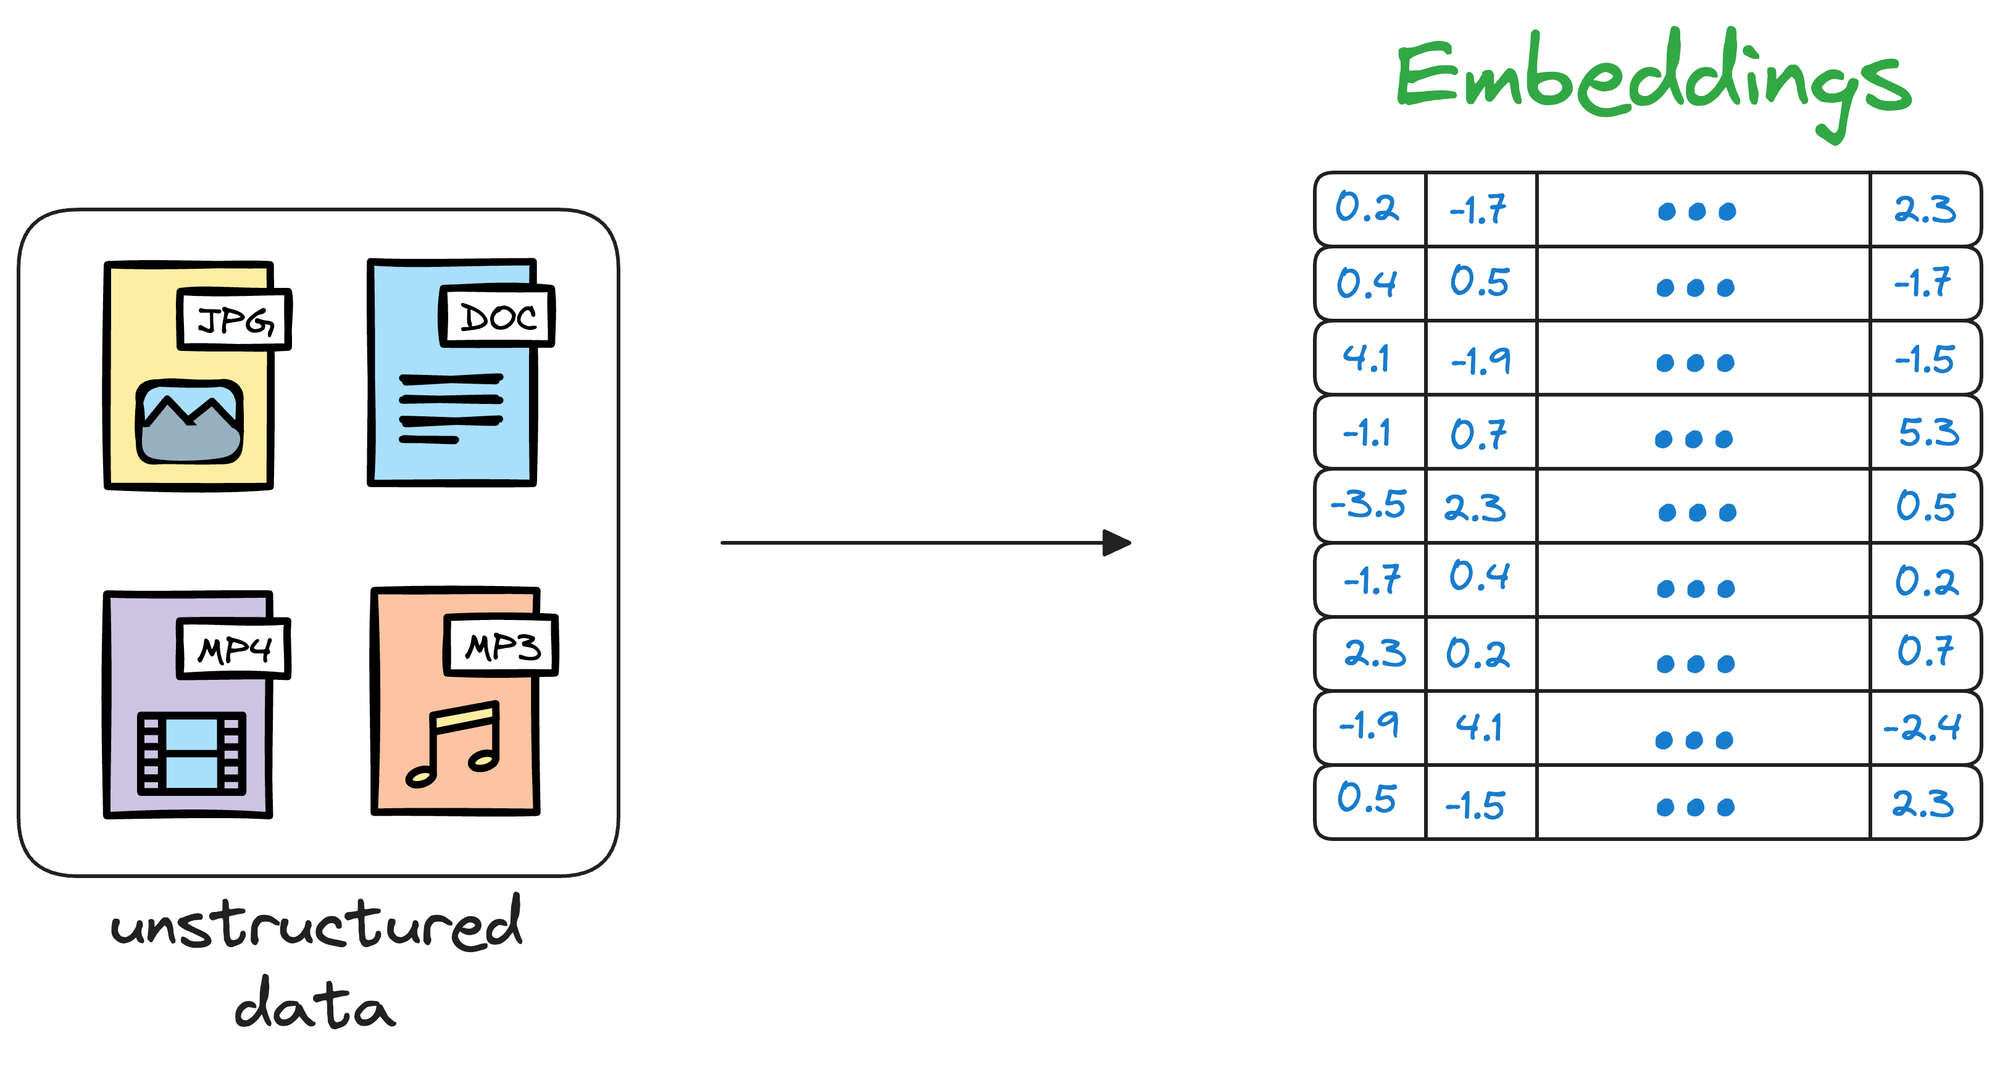
\includegraphics[width=0.6\linewidth,keepaspectratio]{rag42}
		
		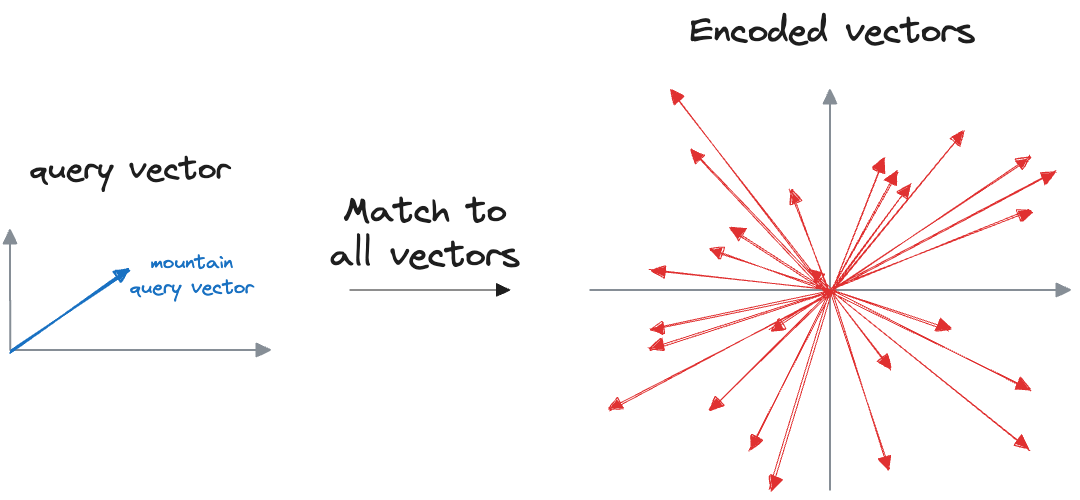
\includegraphics[width=0.6\linewidth,keepaspectratio]{rag43}
		
		\end{center}

{\tiny (Ref: A Crash Course on Building RAG Systems -Daily Dose)}

\end{frame}

%%%%%%%%%%%%%%%%%%%%%%%%%%%%%%%%%%%%%%%%%%%%%%%%%%%%%%%%%%%
\begin{frame}[fragile]\frametitle{Vector Databases}


		\begin{center}
		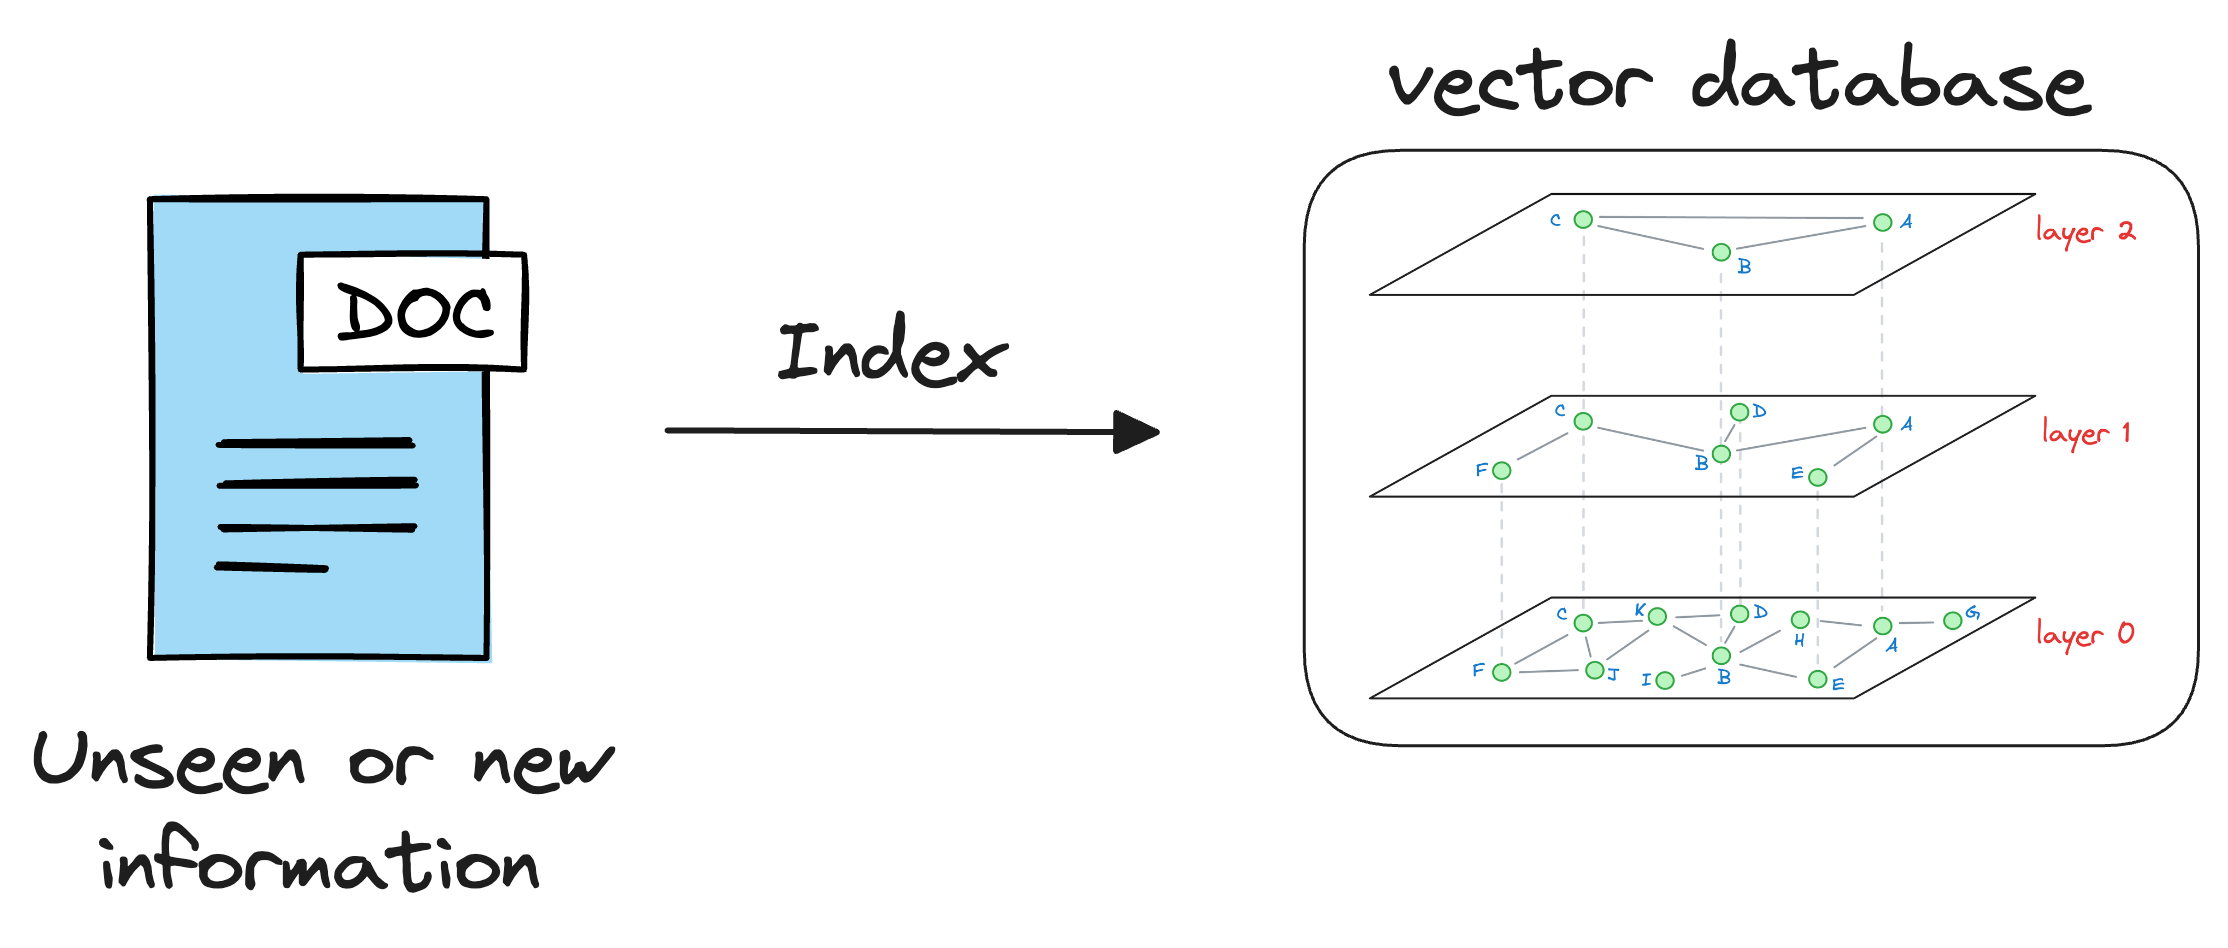
\includegraphics[width=0.6\linewidth,keepaspectratio]{rag46}
		
		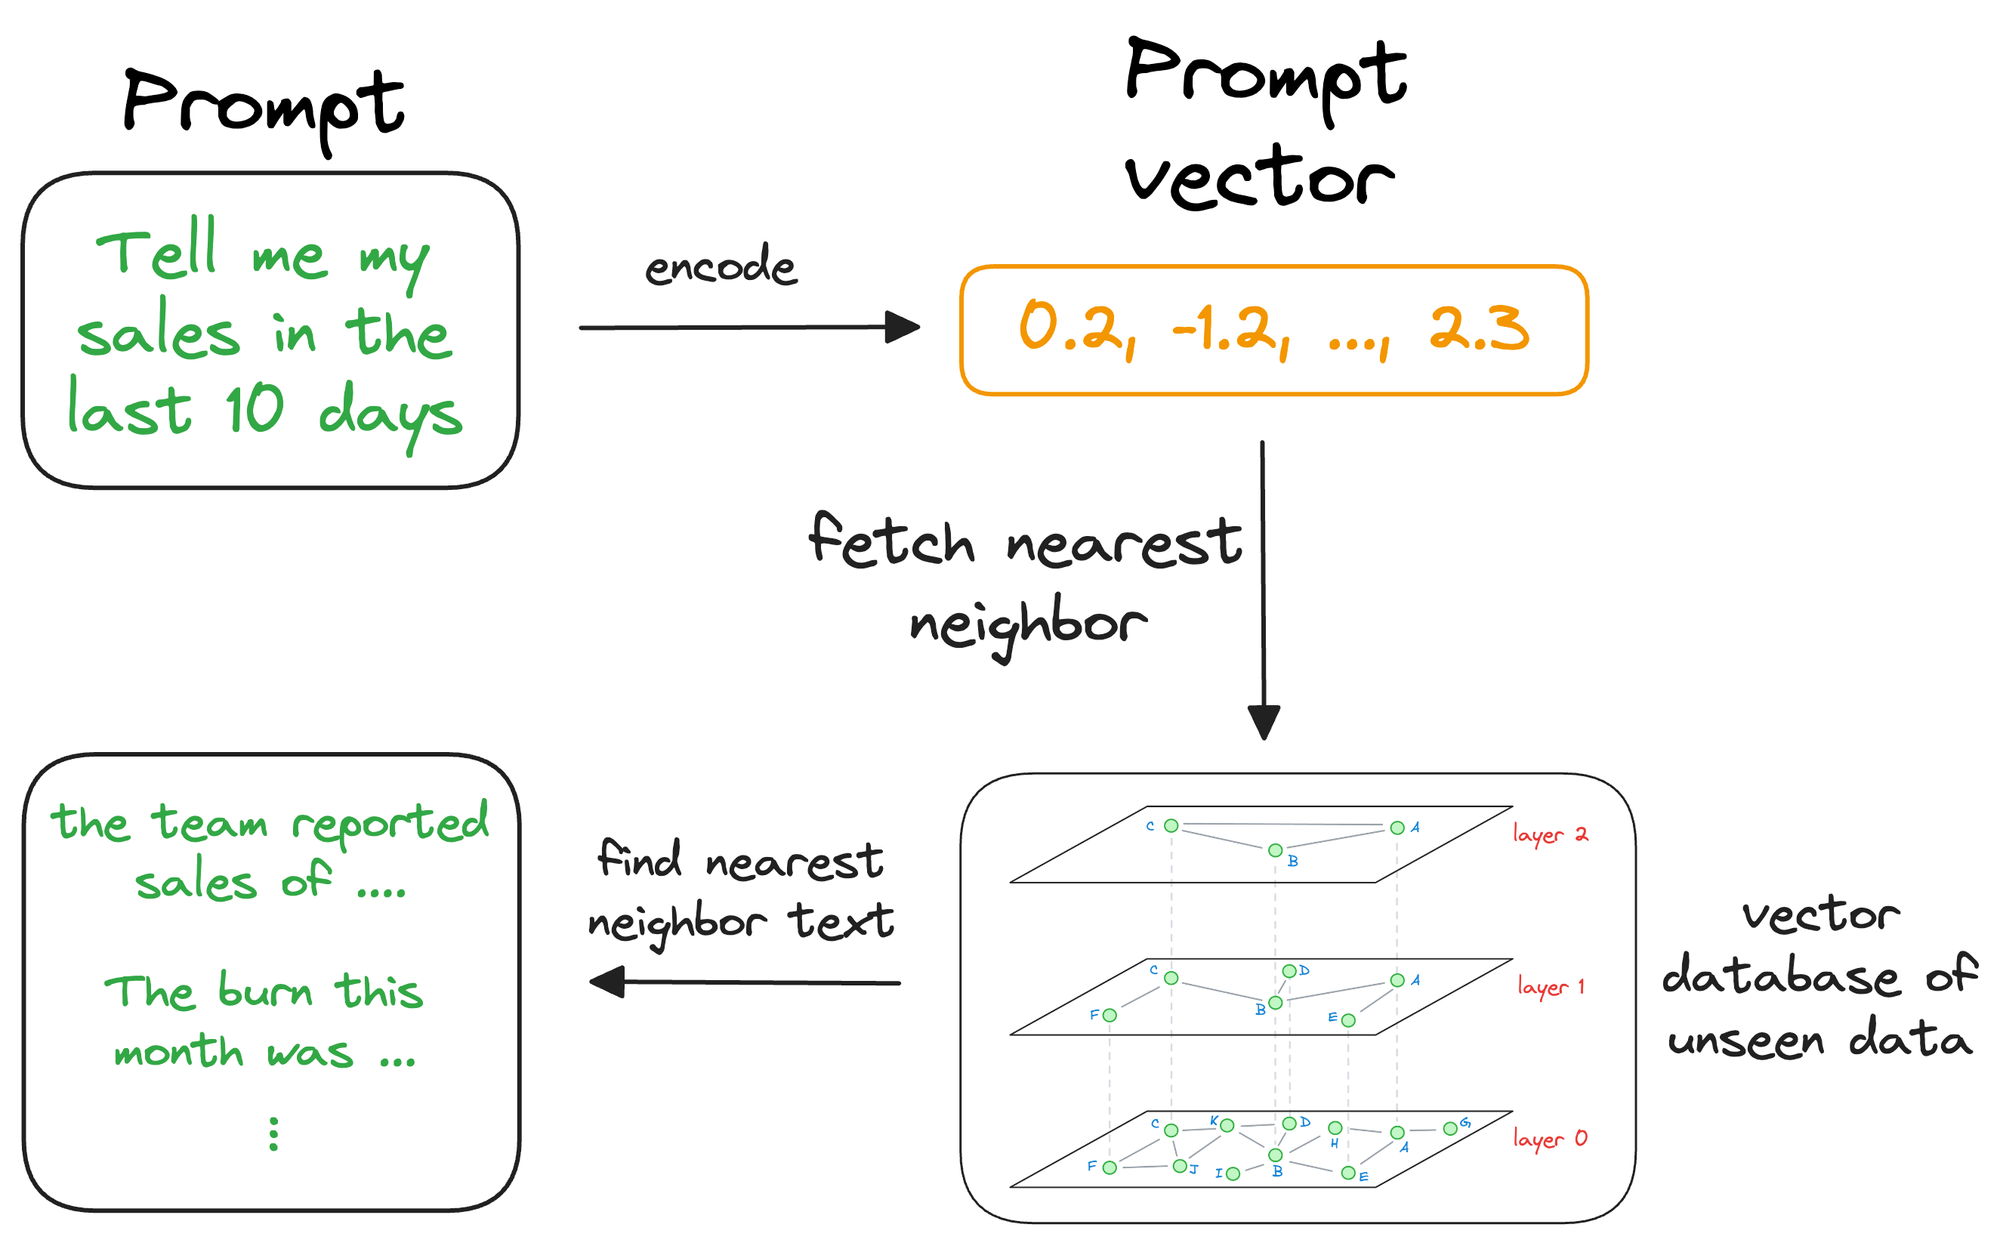
\includegraphics[width=0.6\linewidth,keepaspectratio]{rag47}
		
		\end{center}

{\tiny (Ref: A Crash Course on Building RAG Systems -Daily Dose)}

\end{frame}

%%%%%%%%%%%%%%%%%%%%%%%%%%%%%%%%%%%%%%%%%%%%%%%%%%%%%%%%%%%
\begin{frame}[fragile]\frametitle{Query}



		\begin{center}
		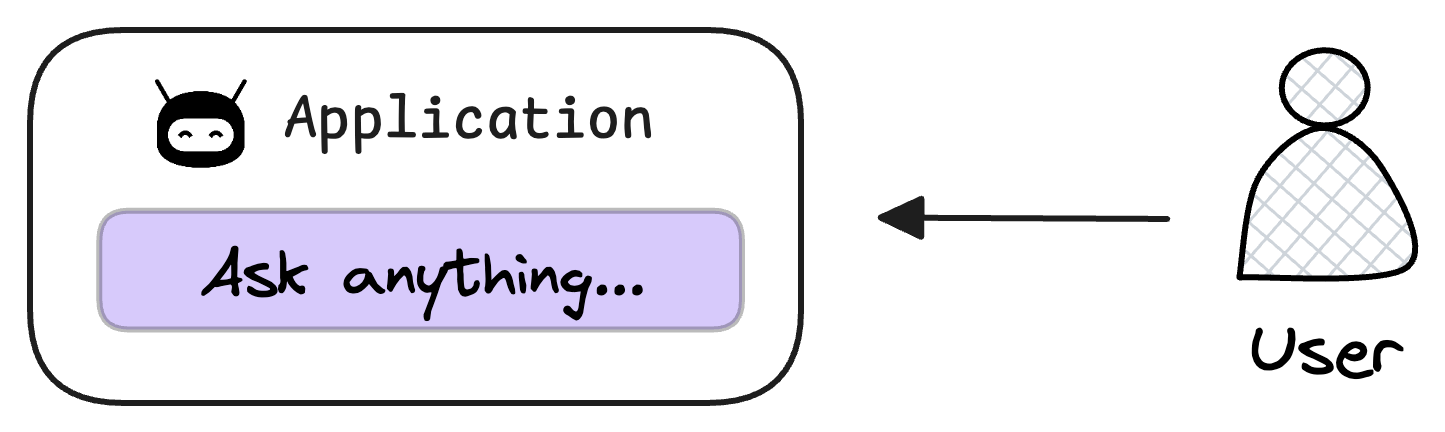
\includegraphics[width=0.8\linewidth,keepaspectratio]{rag55}
		
		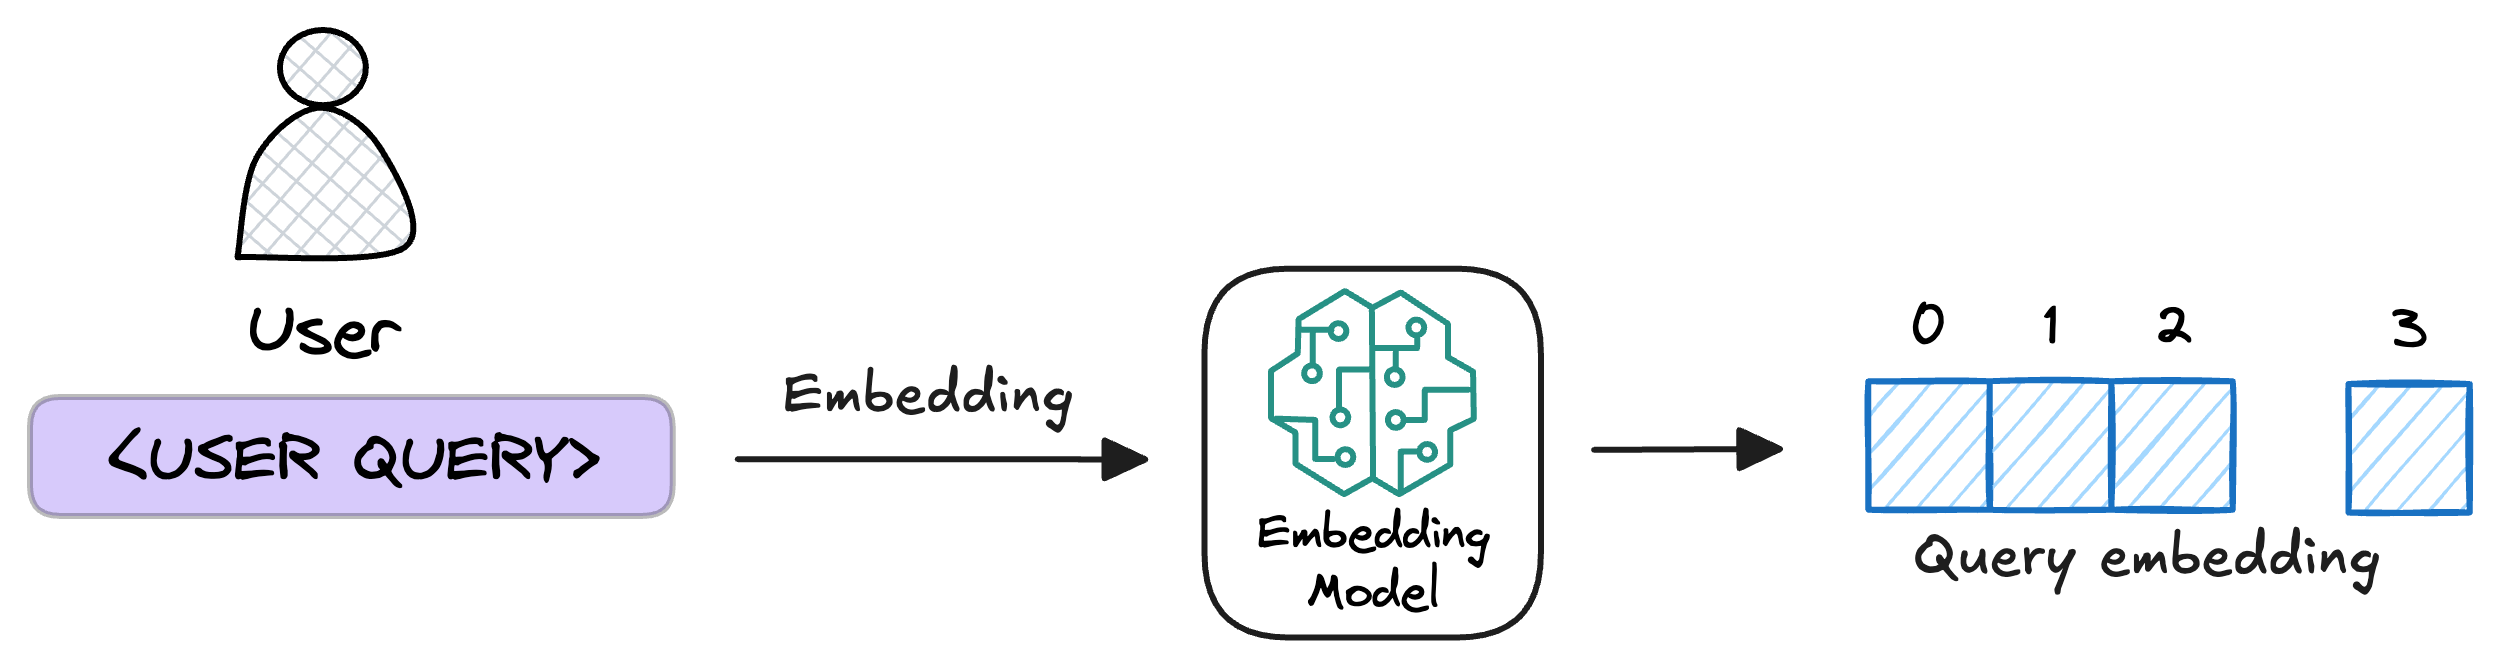
\includegraphics[width=0.8\linewidth,keepaspectratio]{rag56}
		
		\end{center}

{\tiny (Ref: A Crash Course on Building RAG Systems -Daily Dose)}


\end{frame}

%%%%%%%%%%%%%%%%%%%%%%%%%%%%%%%%%%%%%%%%%%%%%%%%%%%%%%%%%%%
\begin{frame}[fragile]\frametitle{Retrieve similar chunks}



		\begin{center}
		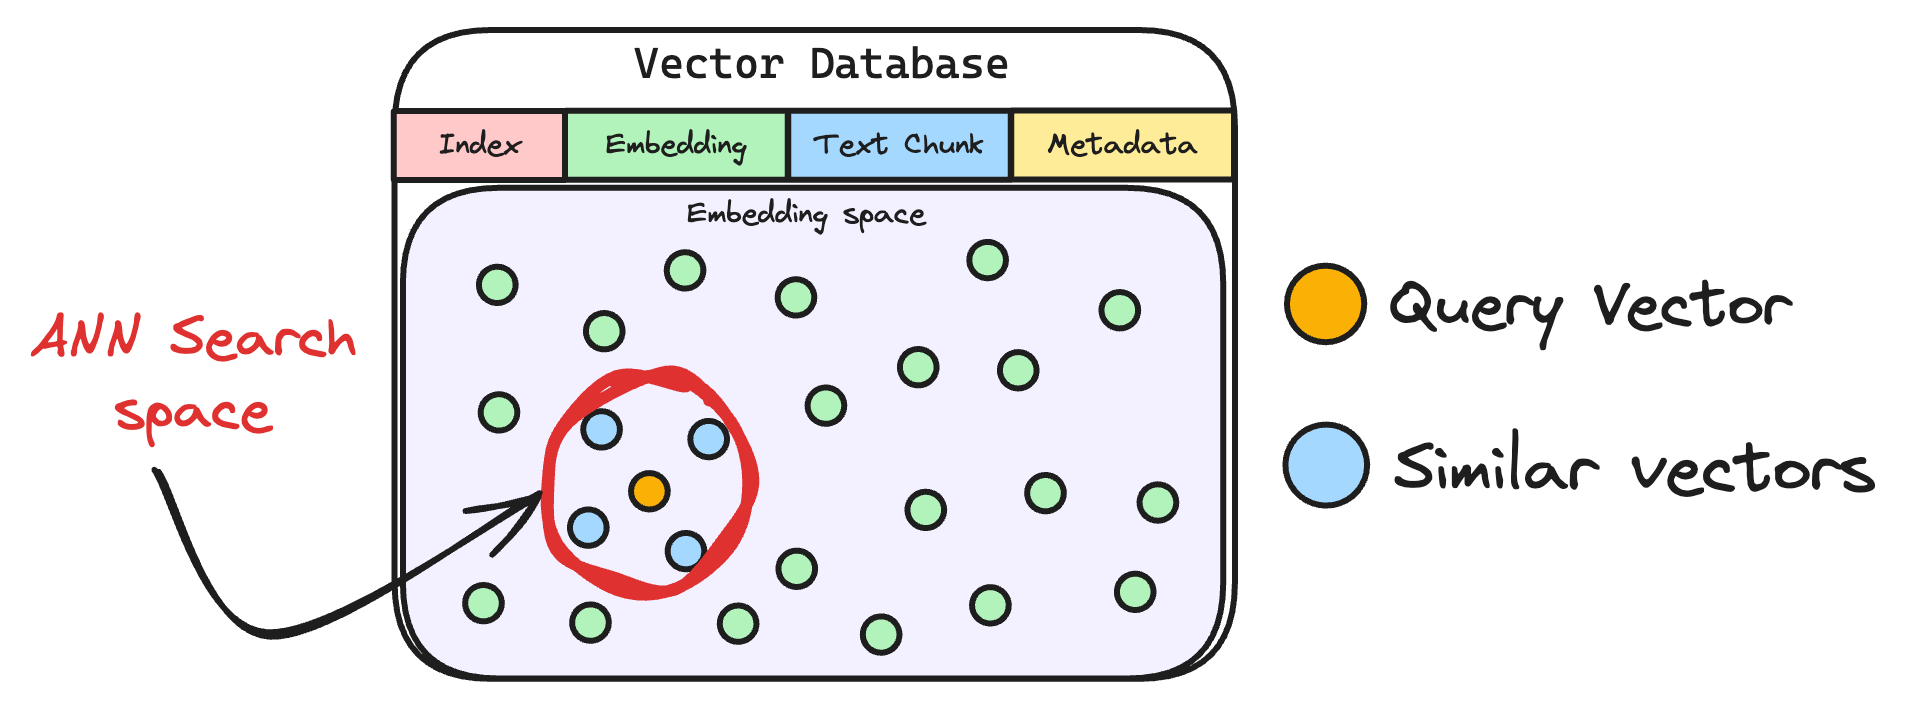
\includegraphics[width=0.8\linewidth,keepaspectratio]{rag57}
		
		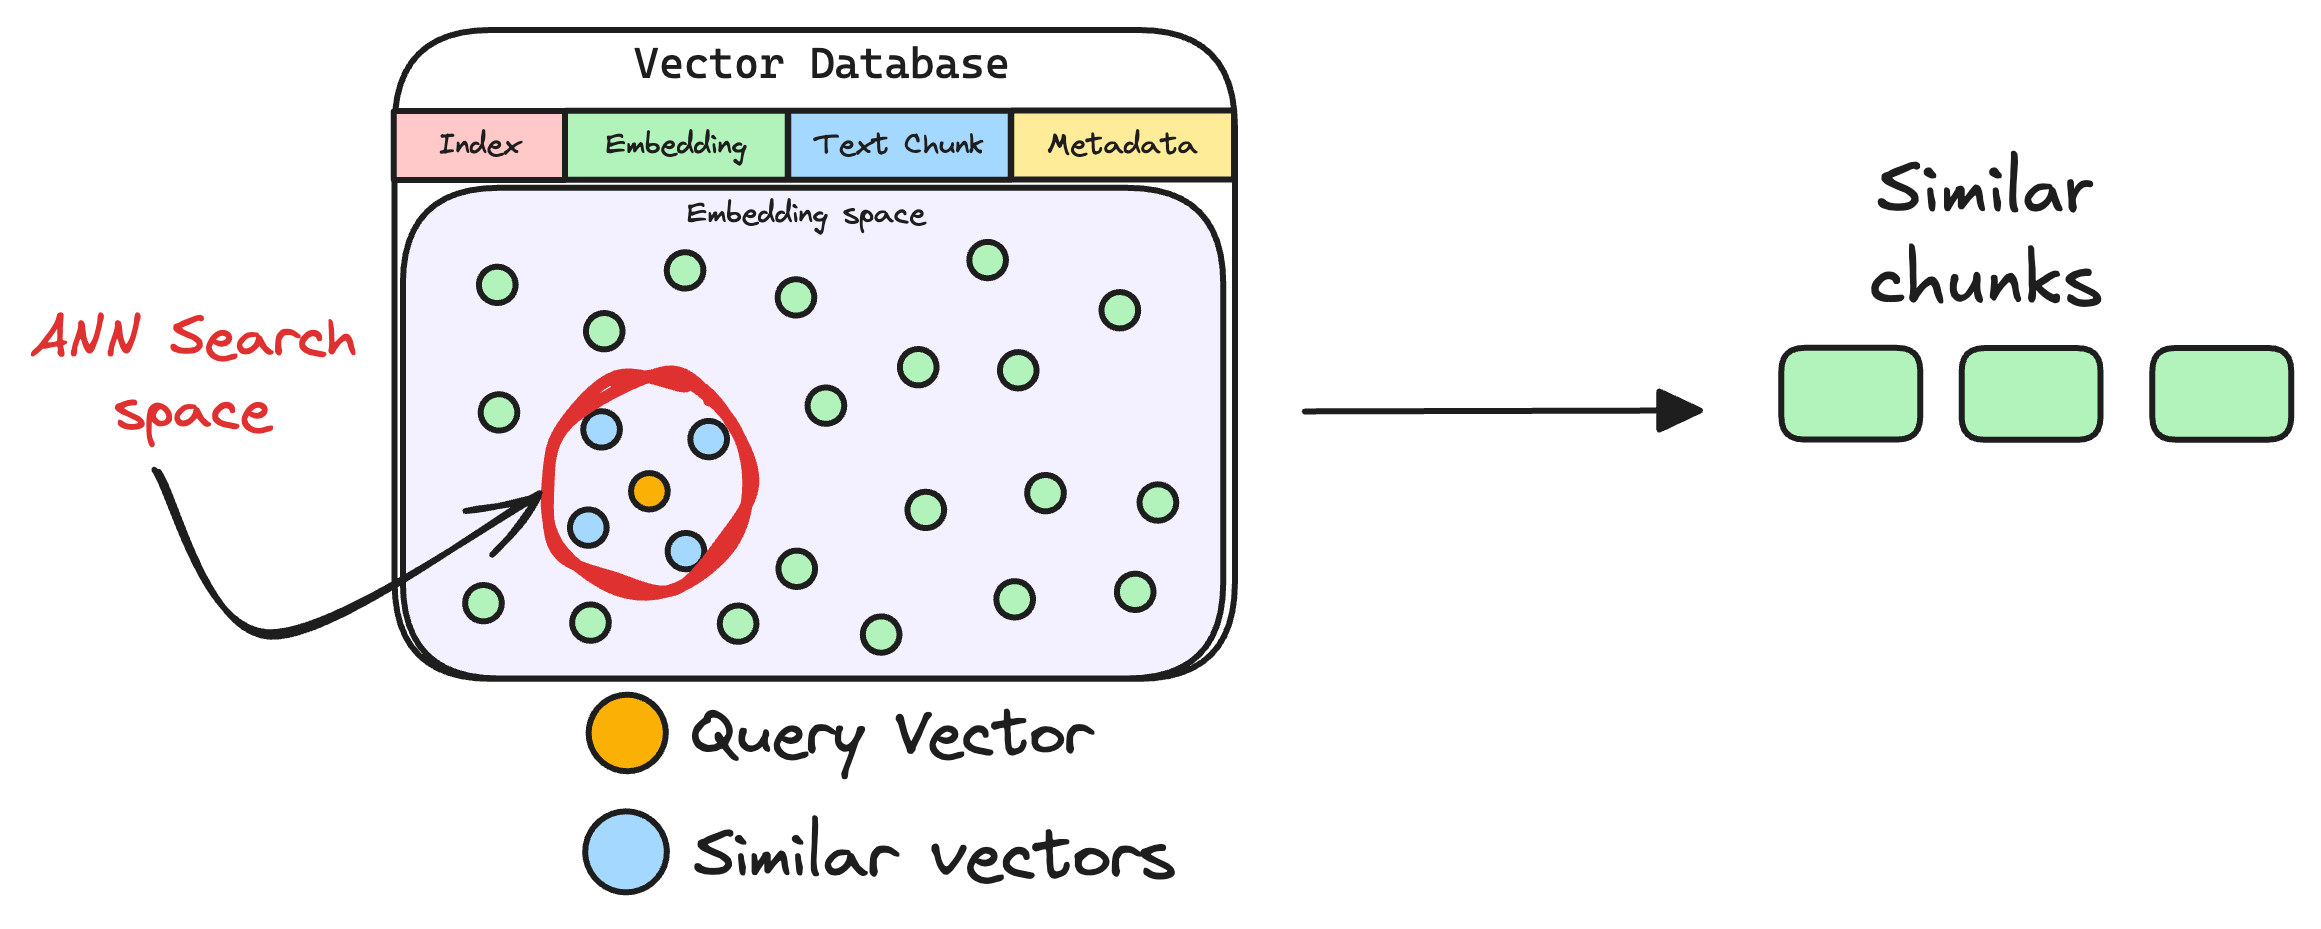
\includegraphics[width=0.8\linewidth,keepaspectratio]{rag58}
		
		\end{center}

{\tiny (Ref: A Crash Course on Building RAG Systems -Daily Dose)}


\end{frame}

%%%%%%%%%%%%%%%%%%%%%%%%%%%%%%%%%%%%%%%%%%%%%%%%%%%%%%%%%%%
\begin{frame}[fragile]\frametitle{Re-rank the chunks}



		\begin{center}
		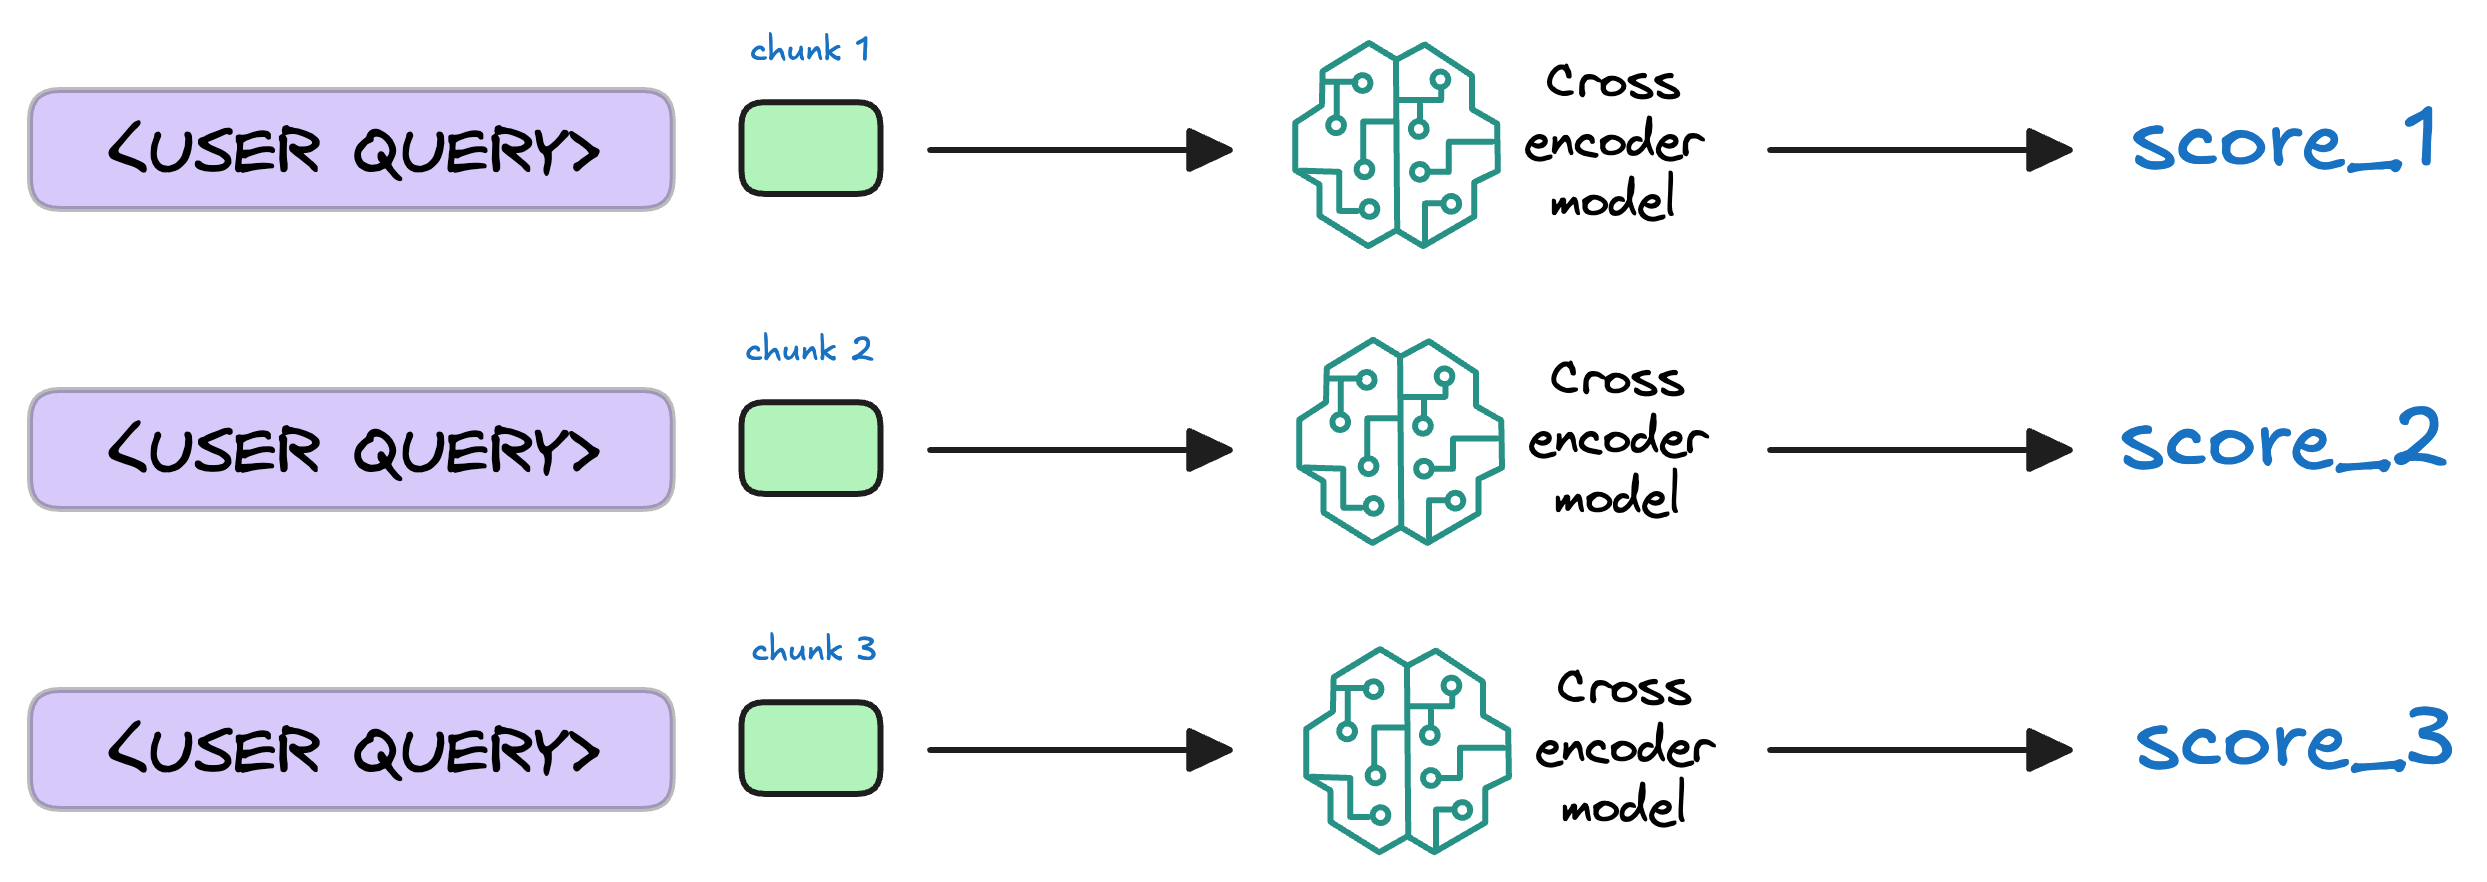
\includegraphics[width=\linewidth,keepaspectratio]{rag59}
		
	
		\end{center}

{\tiny (Ref: A Crash Course on Building RAG Systems -Daily Dose)}


\end{frame}

%%%%%%%%%%%%%%%%%%%%%%%%%%%%%%%%%%%%%%%%%%%%%%%%%%%%%%%%%%%
\begin{frame}[fragile]\frametitle{Generate the final response}



		\begin{center}
		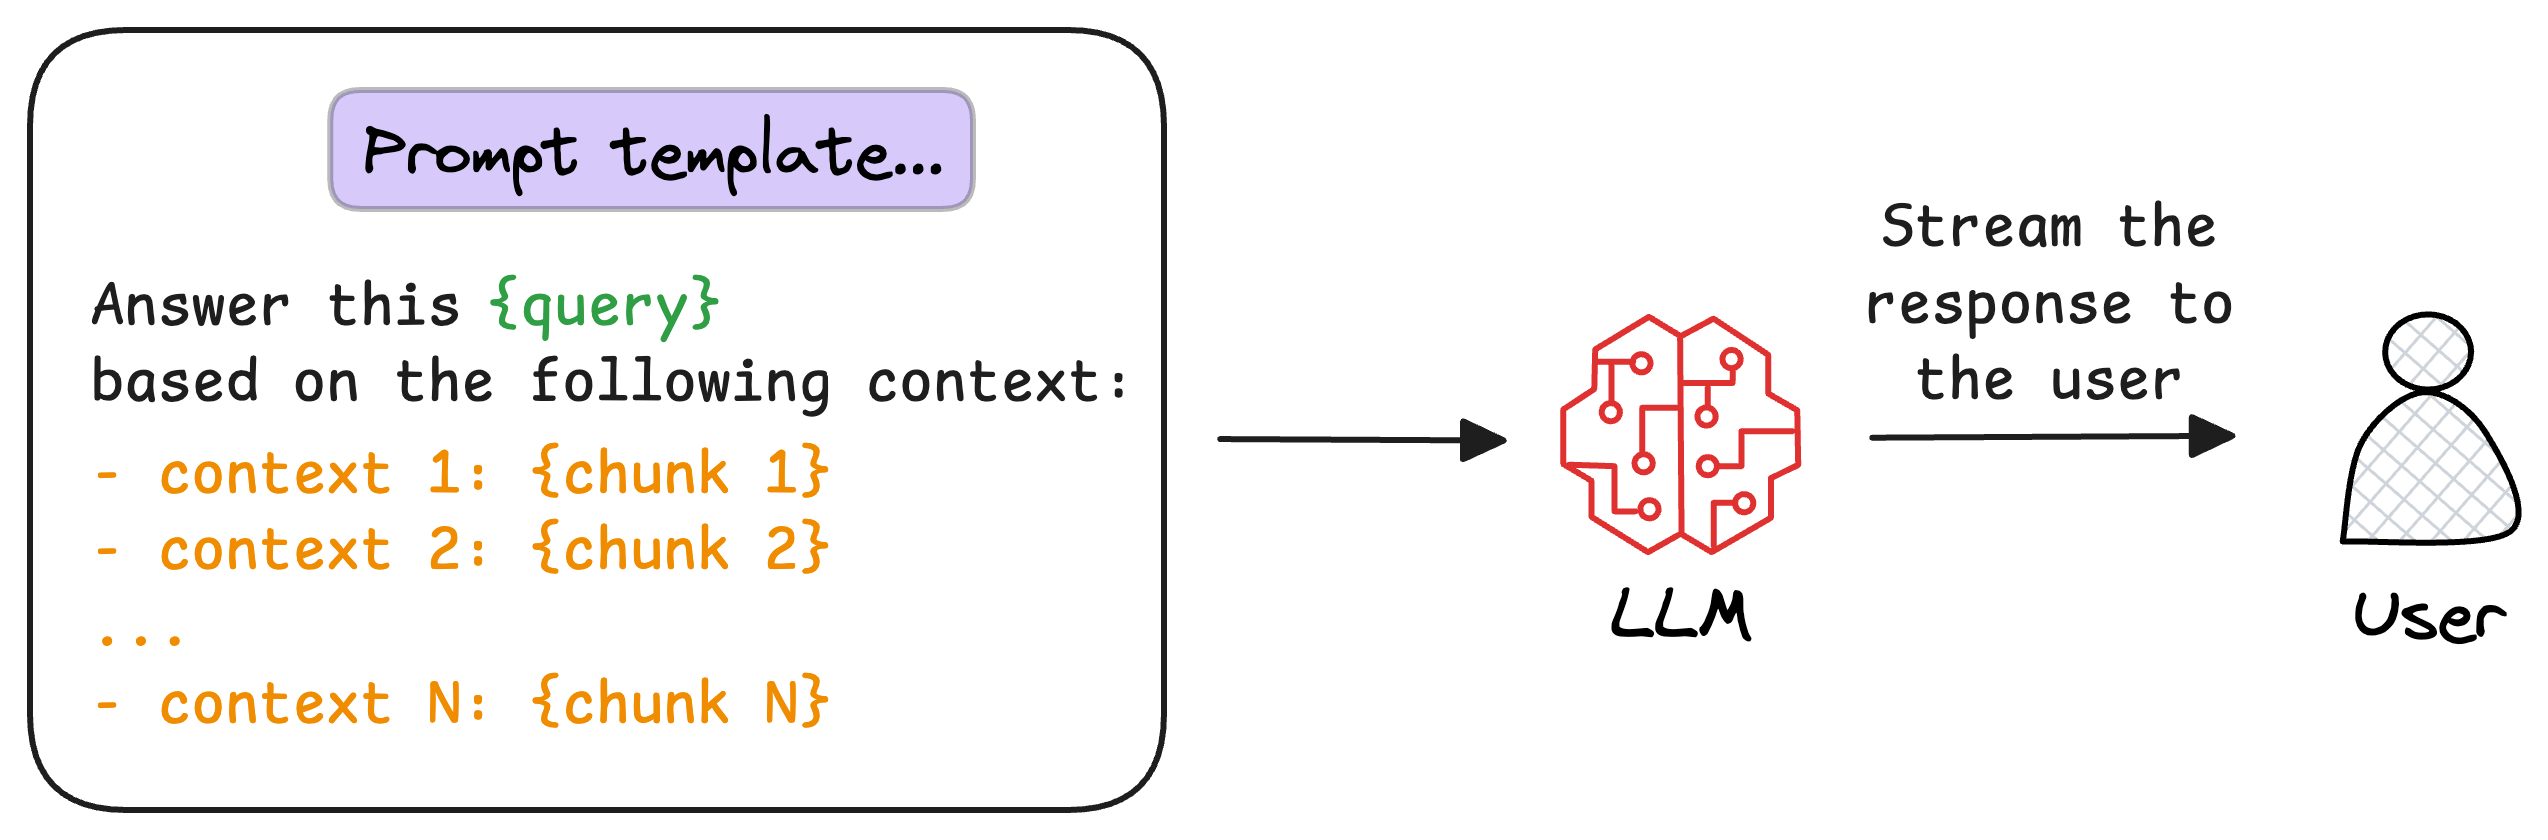
\includegraphics[width=\linewidth,keepaspectratio]{rag60}
		
	
		\end{center}

{\tiny (Ref: A Crash Course on Building RAG Systems -Daily Dose)}


\end{frame}


% %%%%%%%%%%%%%%%%%%%%%%%%%%%%%%%%%%%%%%%%%%%%%%%%%%%%%%%%%%%
% \begin{frame}[fragile]\frametitle{Metrics for RAG evaluation}



		% \begin{center}
		% 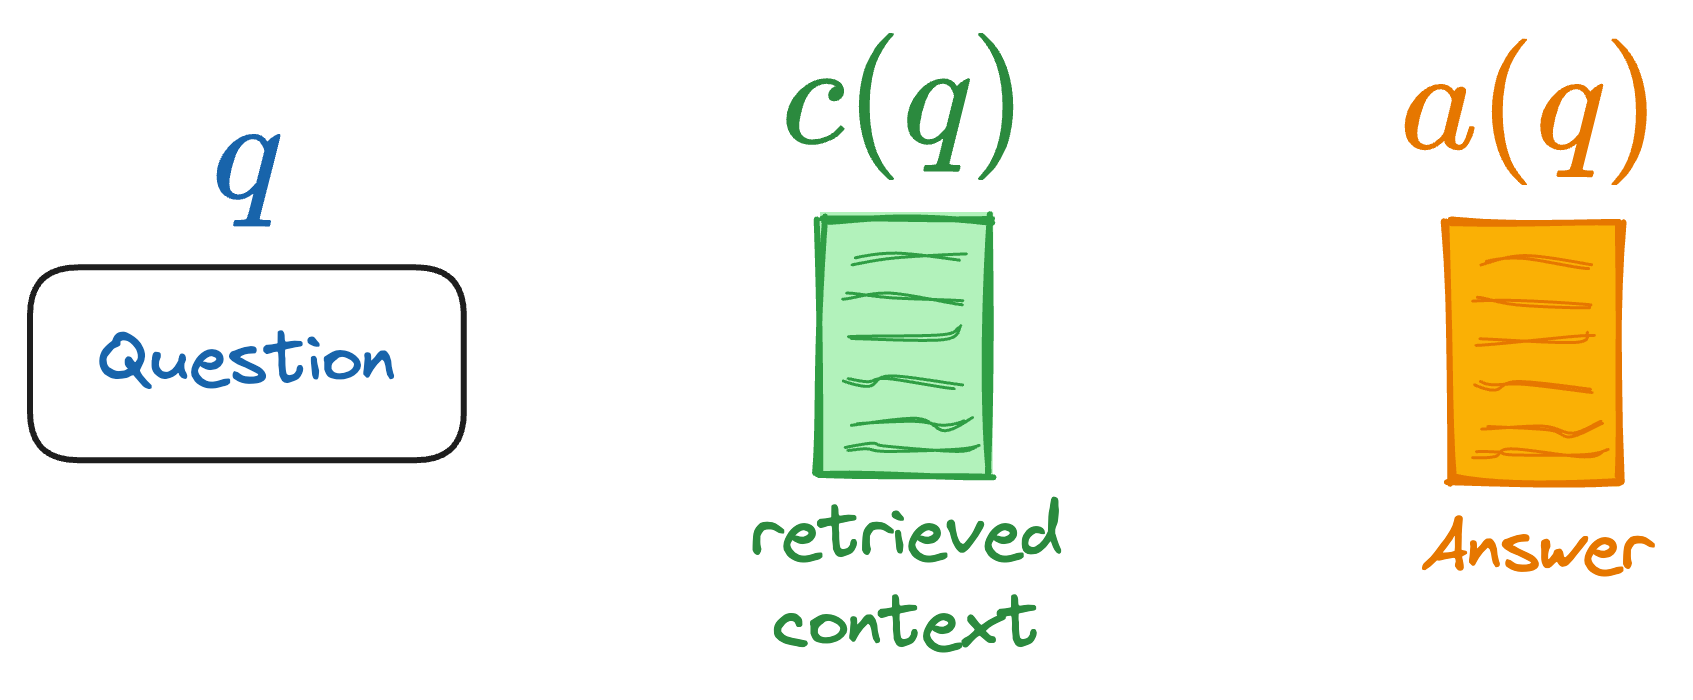
\includegraphics[width=0.8\linewidth,keepaspectratio]{rag61}
		
	
		% \end{center}

% {\tiny (Ref: A Crash Course on Building RAG Systems -Daily Dose)}


% \end{frame}

% %%%%%%%%%%%%%%%%%%%%%%%%%%%%%%%%%%%%%%%%%%%%%%%%%%%%%%%%%%%
% \begin{frame}[fragile]\frametitle{RAG in Steps: Ingestion}

% The first step is to convert internal documents into a query-friendly format by embedding them using an embedding model.

% \begin{itemize}
% \item LLMs can gain external knowledge through information retrieval from memory units like external databases.
% \item There are two types of information retrievers: dense and sparse.
% \item Sparse retrievers use a sparse bag-of-words representation for documents and queries.
% \item Dense (neural) retrievers utilize dense query and document vectors obtained from a neural network.
% \item Retrieval-augmented LMs have shown strong performance in knowledge-intensive tasks, closing the performance gap compared to larger LMs with more parameters.
% \item Save the text representing each embedding along with its corresponding pointer for future reference.
% \end{itemize}

% {\tiny (Ref: Overview of Large Language Models - Aman AI)}

% \end{frame}

% %%%%%%%%%%%%%%%%%%%%%%%%%%%%%%%%%%%%%%%%%%%%%%%%%%%%%%%%%%%
% \begin{frame}[fragile]\frametitle{RAG in Steps: Retrieval}

% Next we can start constructing the answer to a question/query of interest:

% \begin{itemize}
% \item Embed the question using the same Embedding Model as the knowledge base.
% \item Use the resulting Vector Embedding to query the Vector Database and specify the desired number of retrieved vectors, representing the context for answering the query.
% \item Perform an Approximate Nearest Neighbour (ANN) search in the Vector DB to find similar vectors in the Embedding/Latent space.
% \item Map the returned Vector Embeddings to the corresponding text chunks.
% \item Provide the question and retrieved context text chunks to the LLM via prompt, instructing it to use only the provided context for answering the question.
% \item Ensure that prompt engineering is applied to ensure the LLM's answers are within expected boundaries, avoiding fabricated answers when there is no relevant data in the retrieved context.
% \end{itemize}

% {\tiny (Ref: Overview of Large Language Models - Aman AI)}

% \end{frame}


% %%%%%%%%%%%%%%%%%%%%%%%%%%%%%%%%%%%%%%%%%%%%%%%%%%%%%%%%%%%
% \begin{frame}[fragile]\frametitle{RAG in Steps: Generation}


% \begin{itemize}
% \item Next we can start constructing the answer to a question/query of interest
% \item Configuration:
% \begin{itemize}
% \item Temperature: Lower temperature values increase determinism, selecting the highest probable next token. Higher values introduce more randomness, encouraging diversity and creativity in outputs. Lower temperature can be suitable for fact-based QA, while higher temperature may benefit creative tasks like poem generation.
% \item Top\_p: Using nucleus sampling, top\_p controls the determinism of the model's response generation. Lower values prioritize exact and factual answers, while higher values promote diverse responses.
% \end{itemize}

% \item It is generally recommended to modify only one parameter at a time.
% \item Results may vary depending on the specific version of the LLM used.
% \end{itemize}


% {\tiny (Ref: Overview of Large Language Models - Aman AI)}

% \end{frame}

% %%%%%%%%%%%%%%%%%%%%%%%%%%%%%%%%%%%%%%%%%%%%%%%%%%%%%%%%%%%
% \begin{frame}[fragile]\frametitle{Frameworks}

% \begin{itemize}
% \item Employ vector databases like Pinecone, Chroma, Weaviate, Milvus, or LlamaIndex to augment LLMs.
% % \item RAG step-by-step process:
	% % \begin{itemize}
	% % \item Chunk, embed, and index documents in a vector database (VDB).
	% % \item Utilize (approximate) nearest neighbor techniques to match the query embedding of the claim advisor.
	% % \item Retrieve the relevant context from the VDB.
	% % \item Augment the LLM's prompt with the retrieved content.
	% % \end{itemize}

% \item Consider LangChain or Google Vertex for prototyping or industrial applications, respectively.
% \item Another approach is leveraging the search engine itself, as demonstrated by WebGPT, which can interact with a web browser, refine queries, navigate webpages, follow links, and cite sources.e within expected boundaries, avoiding fabricated answers when there is no relevant data in the retrieved context.
% \end{itemize}

% {\tiny (Ref: Overview of Large Language Models - Aman AI)}

% \end{frame}

% % %%%%%%%%%%%%%%%%%%%%%%%%%%%%%%%%%%%%%%%%%%%%%%%%%%%%%%%%%%%
% % \begin{frame}[fragile]\frametitle{RAG in Steps}

% % Next we can start constructing the answer to a question/query of interest:

% % \begin{itemize}
% % \item Interact with the LLM through an API or direct interaction when working with prompts.
% % \item Configure parameters to customize prompt results:


% % {\tiny (Ref: Overview of Large Language Models - Aman AI)}

% % \end{frame}

% %%%%%%%%%%%%%%%%%%%%%%%%%%%%%%%%%%%%%%%%%%%%%%%%%%%%%%%%%%%
% \begin{frame}[fragile]\frametitle{Evaluation and Metrics}

% \begin{itemize}
% \item ROUGE for summarization
% \item BLEU for generation
% \item F1-score for question answering
% \item Additional metrics for factual accuracy, diversity, and coherence
% \end{itemize}	

% \end{frame}


% %%%%%%%%%%%%%%%%%%%%%%%%%%%%%%%%%%%%%%%%%%%%%%%%%%%%%%%%%%%%%%%%%%%%%%%%%%%%%%%%%%
% \begin{frame}[fragile]\frametitle{}
% \begin{center}
% {\Large Approaches in Details}
% \end{center}
% \end{frame}

%%%%%%%%%%%%%%%%%%%%%%%%%%%%%%%%%%%%%%%%%%%%%%%%%%%%%%%%%%%
\begin{frame}[fragile]\frametitle{Naive RAG Approach}

Simply retrieve texts and provide to language model as additional context during generation.

\begin{itemize}
\item Concept: Retrieve relevant documents from an external corpus before generation.
\item Steps: 1. Input query/topic. 2. Retrieve documents. 3. Generate summary/response based on retrieved documents.
\item Pros: Simple and effective for factual tasks.
\item Cons: May lack fluency and originality due to heavy reliance on retrieved text.
\end{itemize}	

\begin{center}
\includegraphics[width=0.8\linewidth,keepaspectratio]{rag1}

{\tiny (Ref: Progression of RAG Systems - Abhinav Kimothi )}
\end{center}		

\end{frame}


%%%%%%%%%%%%%%%%%%%%%%%%%%%%%%%%%%%%%%%%%%%%%%%%%%%%%%%%%%%
\begin{frame}[fragile]\frametitle{RAG Architecture}


		\begin{center}
		\includegraphics[width=\linewidth,keepaspectratio]{rag4a}
		\end{center}

{\tiny (Ref: RAG Architecture -Abhinav  Kimothi)}

\end{frame}

%%%%%%%%%%%%%%%%%%%%%%%%%%%%%%%%%%%%%%%%%%%%%%%%%%%%%%%%%%%
\begin{frame}[fragile]\frametitle{RAG Workflow}


		\begin{center}
		\includegraphics[width=\linewidth,keepaspectratio]{rag4b}
		\end{center}

{\tiny (Ref: RAG Architecture -Abhinav  Kimothi)}

\end{frame}


%%%%%%%%%%%%%%%%%%%%%%%%%%%%%%%%%%%%%%%%%%%%%%%%%%%%%%%%%%%
\begin{frame}[fragile]\frametitle{Challenges in Naive RAG}

\begin{itemize}
\item Retrieval Quality
	\begin{itemize}
	\item Low Precision leading to Hallucinations/Mid-air drops
	\item Low  Recall  resulting in  missing  relevant info
	\item Outdated information
	\end{itemize}
\item Augmentation
	\begin{itemize}
	\item Redundancy and Repetition when multiple retrieved documents have similar information
	\item Context Length challenges
	\end{itemize}
\item Generation Quality
	\begin{itemize}
	\item Generations are not grounded in the context 
	\item Potential of toxicity and bias in the response
	\item Excessive dependence on augmented context
	\end{itemize}
\end{itemize}	


{\tiny (Ref: Progression of RAG Systems - Abhinav Kimothi )}

\end{frame}

% %%%%%%%%%%%%%%%%%%%%%%%%%%%%%%%%%%%%%%%%%%%%%%%%%%%%%%%%%%%
% \begin{frame}[fragile]\frametitle{Modular RAG Architectures}

% Separate retriever and generator modules that can be independently improved.

% \begin{itemize}
% \item Decomposed Modules: Separate modules for retrieval, filtering, and generation, allowing for customization.
% \item Allows components like search, memory, and reranking modules to be configured
% \item Fine-tuning Flexibility: Adapting individual modules to specific tasks or data domains.
% \item Interpretability Advantages: Easier to analyze the contribution of each module to the final output.
% \end{itemize}	

% \end{frame}



% %%%%%%%%%%%%%%%%%%%%%%%%%%%%%%%%%%%%%%%%%%%%%%%%%%%%%%%%%%%
% \begin{frame}[fragile]\frametitle{Modular RAG Architectures}

% \begin{center}
% \includegraphics[width=0.8\linewidth,keepaspectratio]{rag3}

% {\tiny (Ref: Progression of RAG Systems - Abhinav Kimothi )}
% \end{center}

% \end{frame}

% %%%%%%%%%%%%%%%%%%%%%%%%%%%%%%%%%%%%%%%%%%%%%%%%%%%%%%%%%%%
% \begin{frame}[fragile]\frametitle{Some RAG Modules}

  % \begin{itemize}
    % \item \textbf{Search:}
          % \begin{itemize}
              % \item Perform search on different data sources
              % \item Customized for various data sources
              % \item Increase source data for better response generation
          % \end{itemize}
    % \item \textbf{Memory:}
          % \begin{itemize}
              % \item Leverage parametric memory capabilities of the Language Model (LLM)
              % \item Guide retrieval using retrieval-enhanced generator
              % \item Create an unbounded memory pool iteratively
          % \end{itemize}
    % \item \textbf{Fusion (RAG-Fusion):}
          % \begin{itemize}
              % \item Overcome limitations of traditional search systems
              % \item Multi-query approach, expanding user queries into diverse perspectives
              % \item Conduct parallel vector searches for original and expanded queries
              % \item Intelligently re-rank and optimize results
          % \end{itemize}
    % \item \textbf{Extra Generation:}
          % \begin{itemize}
              % \item Generate context using Language Model (LLM)
              % \item Address issues of repetition and irrelevant details in retrieved content
          % \end{itemize}
    % \item \textbf{Task Adaptable Module:}
          % \begin{itemize}
              % \item Make RAG adaptable to various downstream tasks
              % \item Develop task-specific end-to-end retrievers with minimal examples
              % \item Demonstrate flexibility in handling different tasks
          % \end{itemize}
  % \end{itemize}

% \end{frame}

% %%%%%%%%%%%%%%%%%%%%%%%%%%%%%%%%%%%%%%%%%%%%%%%%%%%%%%%%%%%
% \begin{frame}[fragile]\frametitle{Further RAG Variants and Advancements}

% \begin{itemize}
% \item Dense Passage Retrieval
% \item Transformer-based RAG models
% \item Multi-stage RAG with diverse retrieval strategies
% \item Explainable RAG for interpretability
% \item RAG for low-resource languages
% \end{itemize}	

% \end{frame}


%%%%%%%%%%%%%%%%%%%%%%%%%%%%%%%%%%%%%%%%%%%%%%%%%%%%%%%%%%%%%%%%%%%%%%%%%%%%%%%%%%
\begin{frame}[fragile]\frametitle{}
\begin{center}
{\Large RAG vs SFT (Supervised Fine - Tuning)}
\end{center}
\end{frame}




%%%%%%%%%%%%%%%%%%%%%%%%%%%%%%%%%%%%%%%%%%%%%%%%%%%%%%%%%%%
\begin{frame}[fragile]\frametitle{RAG \& SFT: Complementary Techniques}
% \begin{itemize}
  % \item RAG \& SFT are complementary, not competing methods.
  % \item RAG enhances non-parametric memory without changing parameters.
  % \item SFT changes parameters, impacting parametric memory.
% \end{itemize}
\textbf{RAG Features}
\begin{itemize}
  \item Connects to dynamic external data sources.
  \item Reduces hallucinations.
  \item Increases transparency in source of information.
  \item Works well with very large foundation models.
  \item Does not impact style, tone, vocabulary.
\end{itemize}
\textbf{SFT Features}
\begin{itemize}
  \item Changes style, vocabulary, tone of foundation model.
  \item Can reduce model size.
  \item Useful for deep domain expertise.
  \item May not address hallucinations.
  \item No improvement in transparency (black box models).
\end{itemize}
\end{frame}

% %%%%%%%%%%%%%%%%%%%%%%%%%%%%%%%%%%%%%%%%%%%%%%%%%%%%%%%%%%%
% \begin{frame}[fragile]\frametitle{Use Case Considerations for RAG \& SFT}
% Use both if parametric and non-parametric memory changes are needed.

% \begin{itemize}
  % \item Access to dynamic external data source.
  % \item Resolving hallucinations.
  % \item Transparency in source of information.
  % \item SFT requires access to labeled training data.
% \end{itemize}
% \end{frame}

%%%%%%%%%%%%%%%%%%%%%%%%%%%%%%%%%%%%%%%%%%%%%%%%%%%%%%%%%%%
\begin{frame}[fragile]\frametitle{Important Use Case Considerations}


		\begin{center}
		\includegraphics[width=0.8\linewidth,keepaspectratio]{rag24}
		\end{center}

{\tiny (Ref: Generative AI with Large Language Model - Abhinav  Kimothi)}

\end{frame}

%%%%%%%%%%%%%%%%%%%%%%%%%%%%%%%%%%%%%%%%%%%%%%%%%%%%%%%%%%%
\begin{frame}[fragile]\frametitle{Other Considerations}
\begin{itemize}
  \item \textbf{Latency:} RAG introduces inherent latency due to search and retrieval.
  \item \textbf{Scalability:} RAG pipelines are modular and scalable; SFT requires retraining.
  \item \textbf{Cost:} Both methods require upfront investment; costs vary.
  \item \textbf{Expertise:} RAG pipelines are moderately simple with frameworks; SFT needs deep understanding and training data creation.
\end{itemize}
\end{frame}


%%%%%%%%%%%%%%%%%%%%%%%%%%%%%%%%%%%%%%%%%%%%%%%%%%%%%%%%%%%%%%%%%%%%%%%%%%%%%%%%%%
\begin{frame}[fragile]\frametitle{}
\begin{center}
{\Large Applications}
\end{center}
\end{frame}


%%%%%%%%%%%%%%%%%%%%%%%%%%%%%%%%%%%%%%%%%%%%%%%%%%%%%%%%%%%
\begin{frame}[fragile]\frametitle{Applications and Use Cases}

\begin{itemize}
\item Code generation in software development
\item Creative writing and storytelling
\item Educational material generation
\item Personalized product descriptions
\item many many more \ldots
\end{itemize}	

\end{frame}


%%%%%%%%%%%%%%%%%%%%%%%%%%%%%%%%%%%%%%%%%%%%%%%%%%%%%%%%%%%
\begin{frame}[fragile]\frametitle{Open Source Resources and Tools}

\begin{itemize}
\item LangChain, LlamaIndex like frameworks
\item Transformers library, Hugging Face model hub
\item Datasets and evaluation benchmarks
\end{itemize}	

\end{frame}

